This section is based on the results of Mariame Maiga's internship for her 1st year of Masters at Sorbonne Université, which I co-supervised with Frédérique Cheruy from April to July 2025. The impact of climate change was studied during the internship but not the effects of irrigation in the future, which was analysed later. All simulations used in this section were run by Frédérique Cheruy. 
Multiple technical issues were encountered to obtain reliable simulations of future climate with and without irrigation, therefore these results remain preliminary.

\hfill

To simulate future climate conditions, the LAM is used with forcing data from a global ICOLMDZOR simulation, under climate change scenario SSP5-8.5, which presents the strongest increase in global mean temperature. The mid-century period 2050-2062 was studied and compared to the present period (2010-2022). Longer simulations are under analysis to extend the study period to 30 years for both present and future but they were not yet available when writing this manuscript.
The smaller LAM domain ($R_{domain} = 1000 km$, $NBP=40$) was used for computational efficiency, considering the findings of Section \ref{sec:forcing} that the inconsistencies on the edges of the domain are limited when the LAM is forced by ICOLMDZOR.

Simulations without irrigation in the present (\presnoirr) and future climate (\futnoirr) are compared to characterize the impacts of climate change over the Peninsula. Then, \futnoirr is compared to a simulation over the same period, with irrigation (\futirr) to analyse how irrigation interacts with these impacts.

\subsection{Impact of climate change over the Iberian Peninsula}

The annual impact of climate change under the SSP5-8.5 scenario on land-atmosphere coupling variables is presented in Fig. \ref{fig:diffmaps_present_future}, as the difference between the \futnoirr (2050-2062) and \presnoirr (2010-2022) simulations. 
%temperature
A general warming of the air is observed, as expected with a strong climate change scenario, with 2-m temperature increases of 2°C in most of the domain and up to 3°C in the northern half of the Peninsula (Fig. \ref{fig:diffmaps_present_future}a). The coasts are slightly less affected by warming, whereas the moutain ranges are the most impacted regions.
%precip
Precipitation decreases over most of the Peninsula, especially in the northern coast and the Pyrenees while the only region where it increases is the Southeast (Fig. \ref{fig:diffmaps_present_future}c). This region usually receives little precipitation so, although the absolute values are small, the relative increase is higher than 10\% over a large area and exceeds 25\% in several grid cells (Fig. \ref{fig:reldiffmaps_present_future}).
%evap and fluxsens
The changes in precipitation translate into similar changes in ET, of lower magnitude (Fig. \ref{fig:diffmaps_present_future}d). The only exceptions are in  Pyrenees and Cantabrian mountain ranges in the North, which are very humid areas where ET is limited by incoming radiation rather than available soil moisture.
The sensible heat flux is increased over almost all the continental domain  (Fig. \ref{fig:diffmaps_present_future}b). This evolution is not only a consequence of changes in surface energy partitionning since increases are also visible in areas where ET is increasing. It is likely dominated by an increase in the incoming energy at the surface, since it closely linked to increases in downwelling shortwave radiation (Fig. \ref{fig:diffmaps_present_future}g).
%q2m and RH2m
Specific humidity at 2m is increased over all the domain, with the largest increases reaching $1 g \cdot kg^{-1}$ on coastal areas (Fig. \ref{fig:diffmaps_present_future}e), which corresponds to a 10\% increase. Considering the increase in 2-m air temperature, this can be understood using the Clausius-Clapeyron relation, showing that warmer air can contain more water. %option:quote IPCC WG1 box on precipitation
However, under climate change, the increase in specific humidity is not as impactful as the increase in temperature since relative humidity at 2m is lower over all the continental domain (Fig. \ref{fig:diffmaps_present_future}f), especially in the North of the Peninsula. 
%link to rad fluxes and cloud cover
This explains the increase in the downwelling shortwave radiation flux (Fig. \ref{fig:diffmaps_present_future}g) since less condensed water is present in the atmosphere, particularly in the Northwest of the Peninsula. 
The general increase in longwave downwelling radiation (Fig. \ref{fig:diffmaps_present_future}h) is the consequence of a warmer atmosphere, but this increase is not as large in the North and Northwest of the domain, which is consistent with a lower relative humidity and cloud cover over these regions. 
%option : cloud cover in Appendix ? (with low, medium, high ?)

%figure : diff maps (no_irr, present - future)
\begin{figure}[htbp]
    \centering
    \begin{tabular}{cc}
        %t2m
        \begin{subfigure}[b]{0.5\textwidth}
            \caption{2-m temperature difference}
            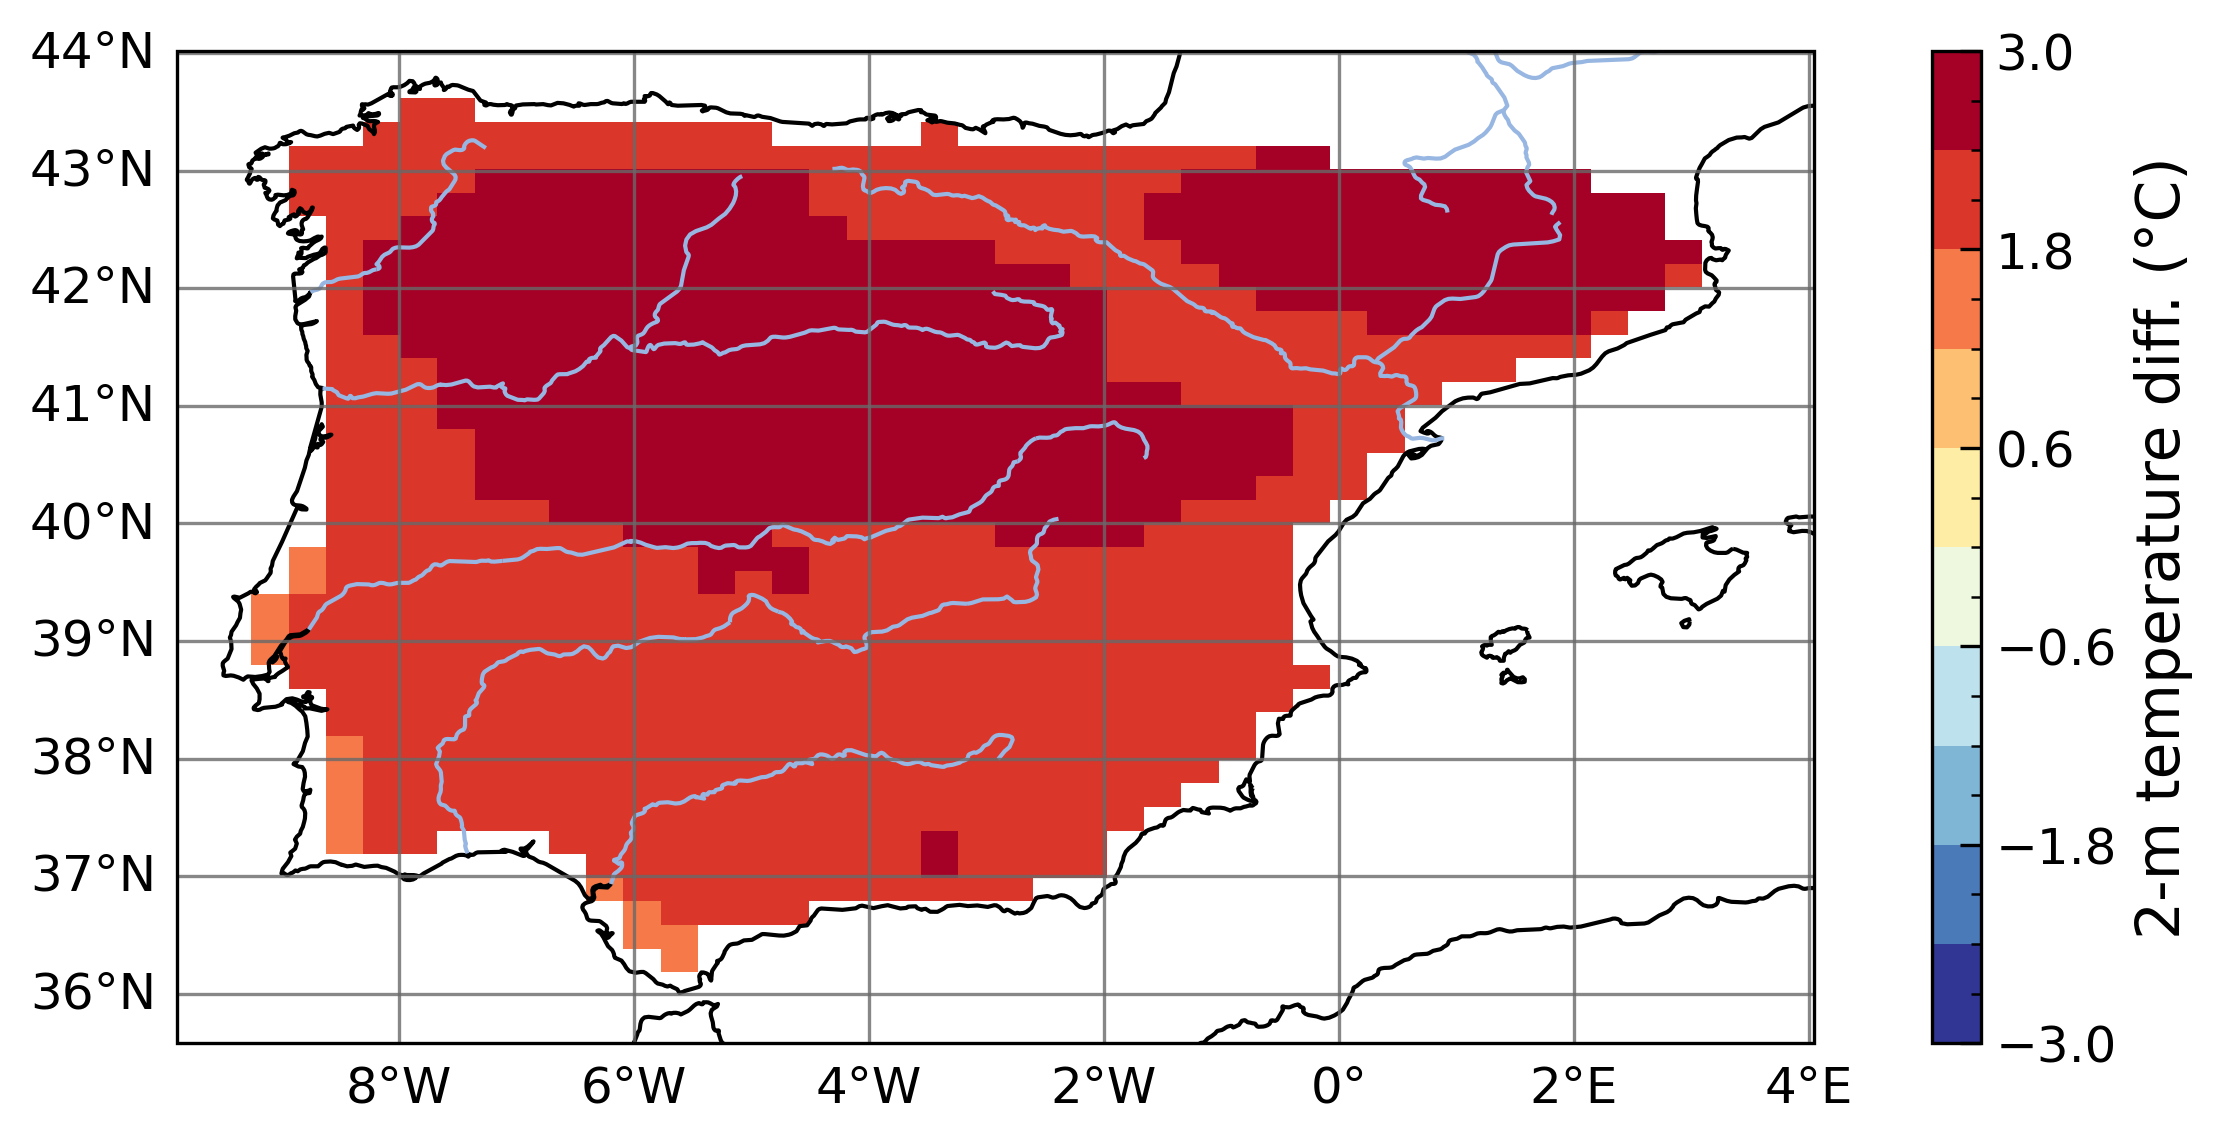
\includegraphics[width=\textwidth]{images/chap4/future/diffmap_t2m_presfut.png}
        \end{subfigure} &
        %fluxsens
        \begin{subfigure}[b]{0.5\textwidth}
            \caption{Sensible heat flux difference}
            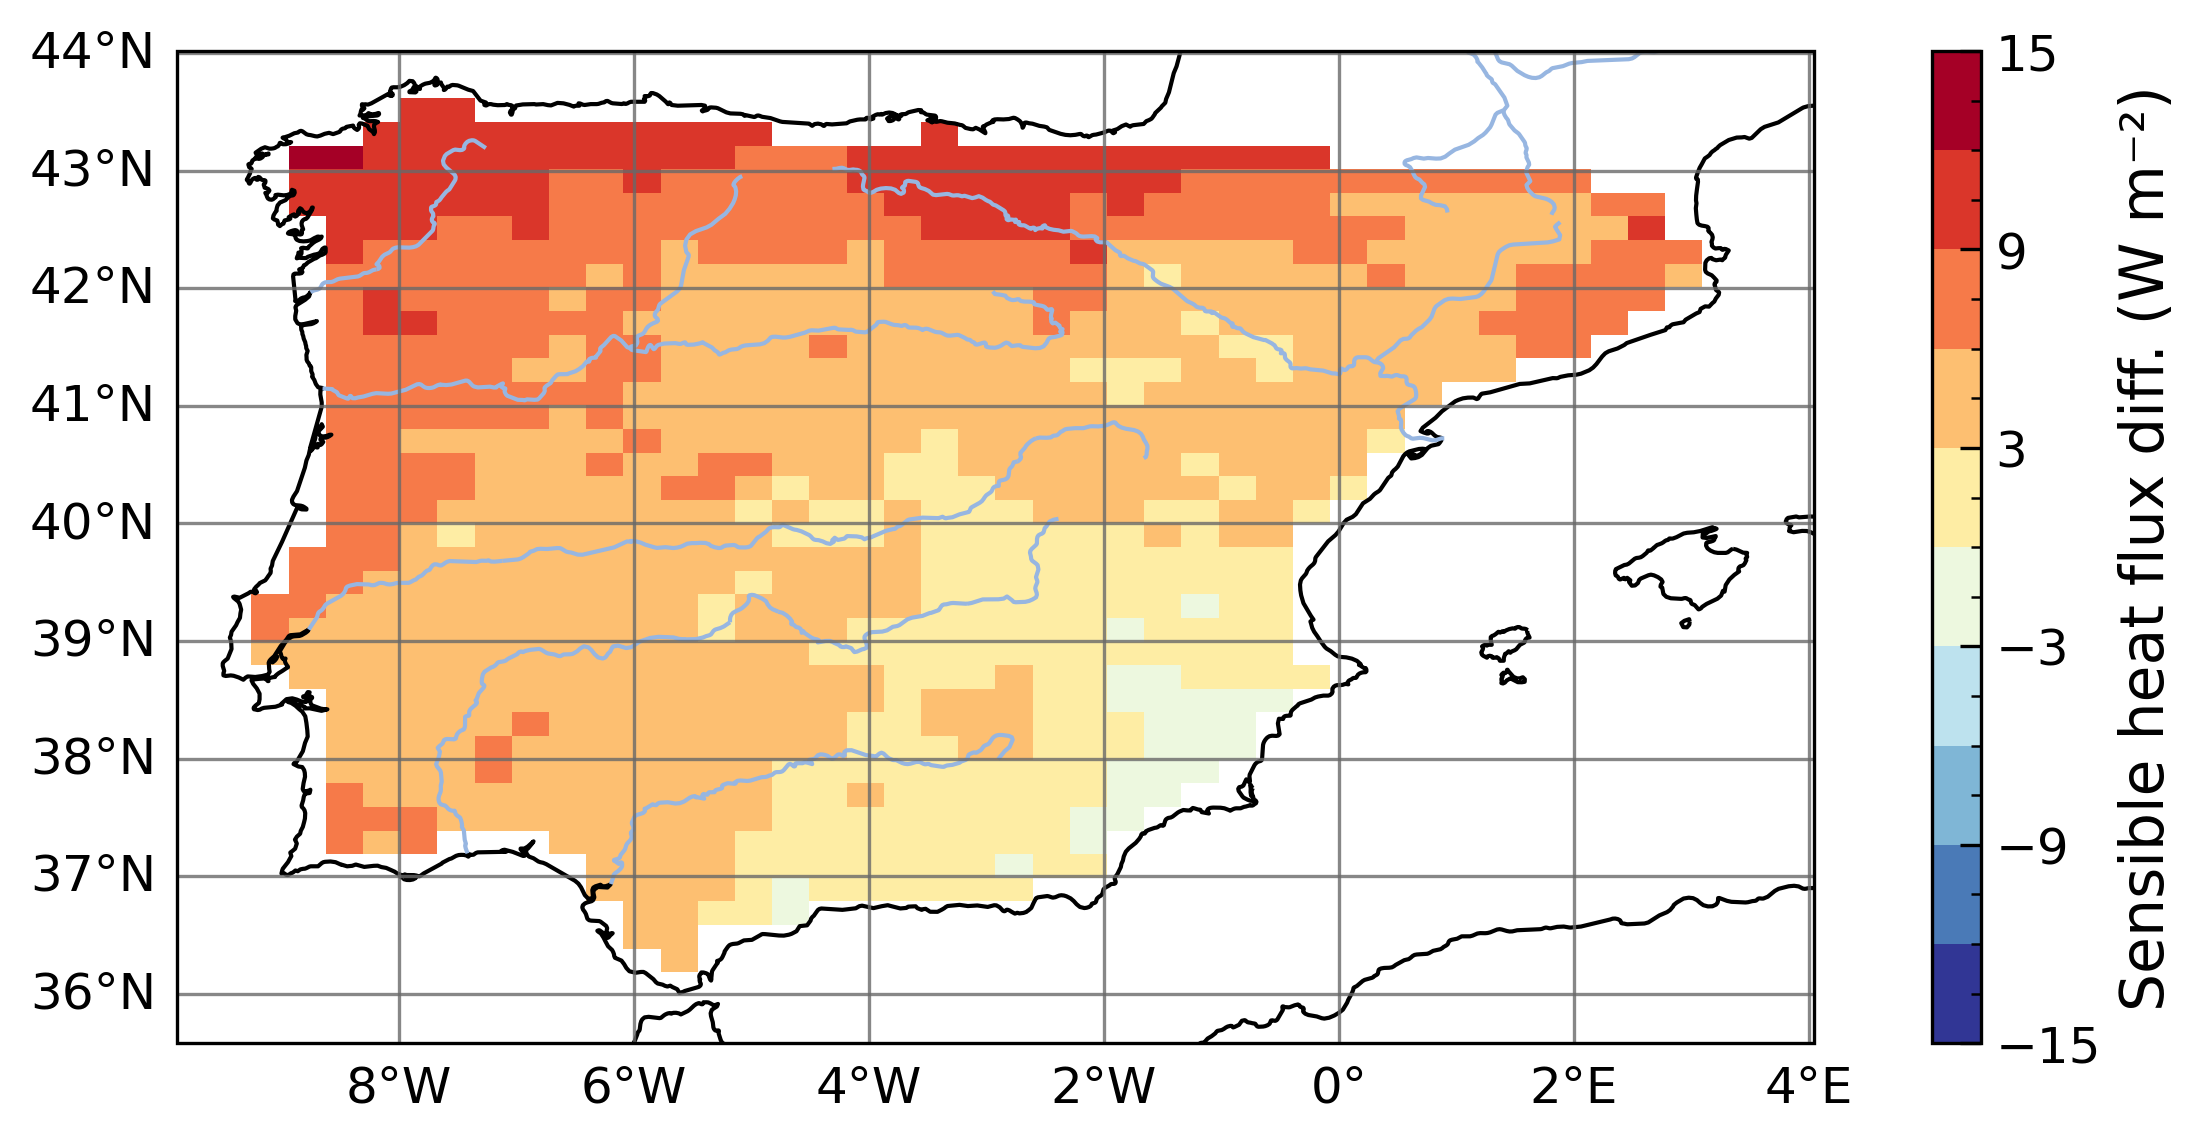
\includegraphics[width=\textwidth]{images/chap4/future/diffmap_fluxsens_presfut.png}
        \end{subfigure} \\
        
        %precip
        \begin{subfigure}[b]{0.5\textwidth}
            \caption{Precipitation difference}
            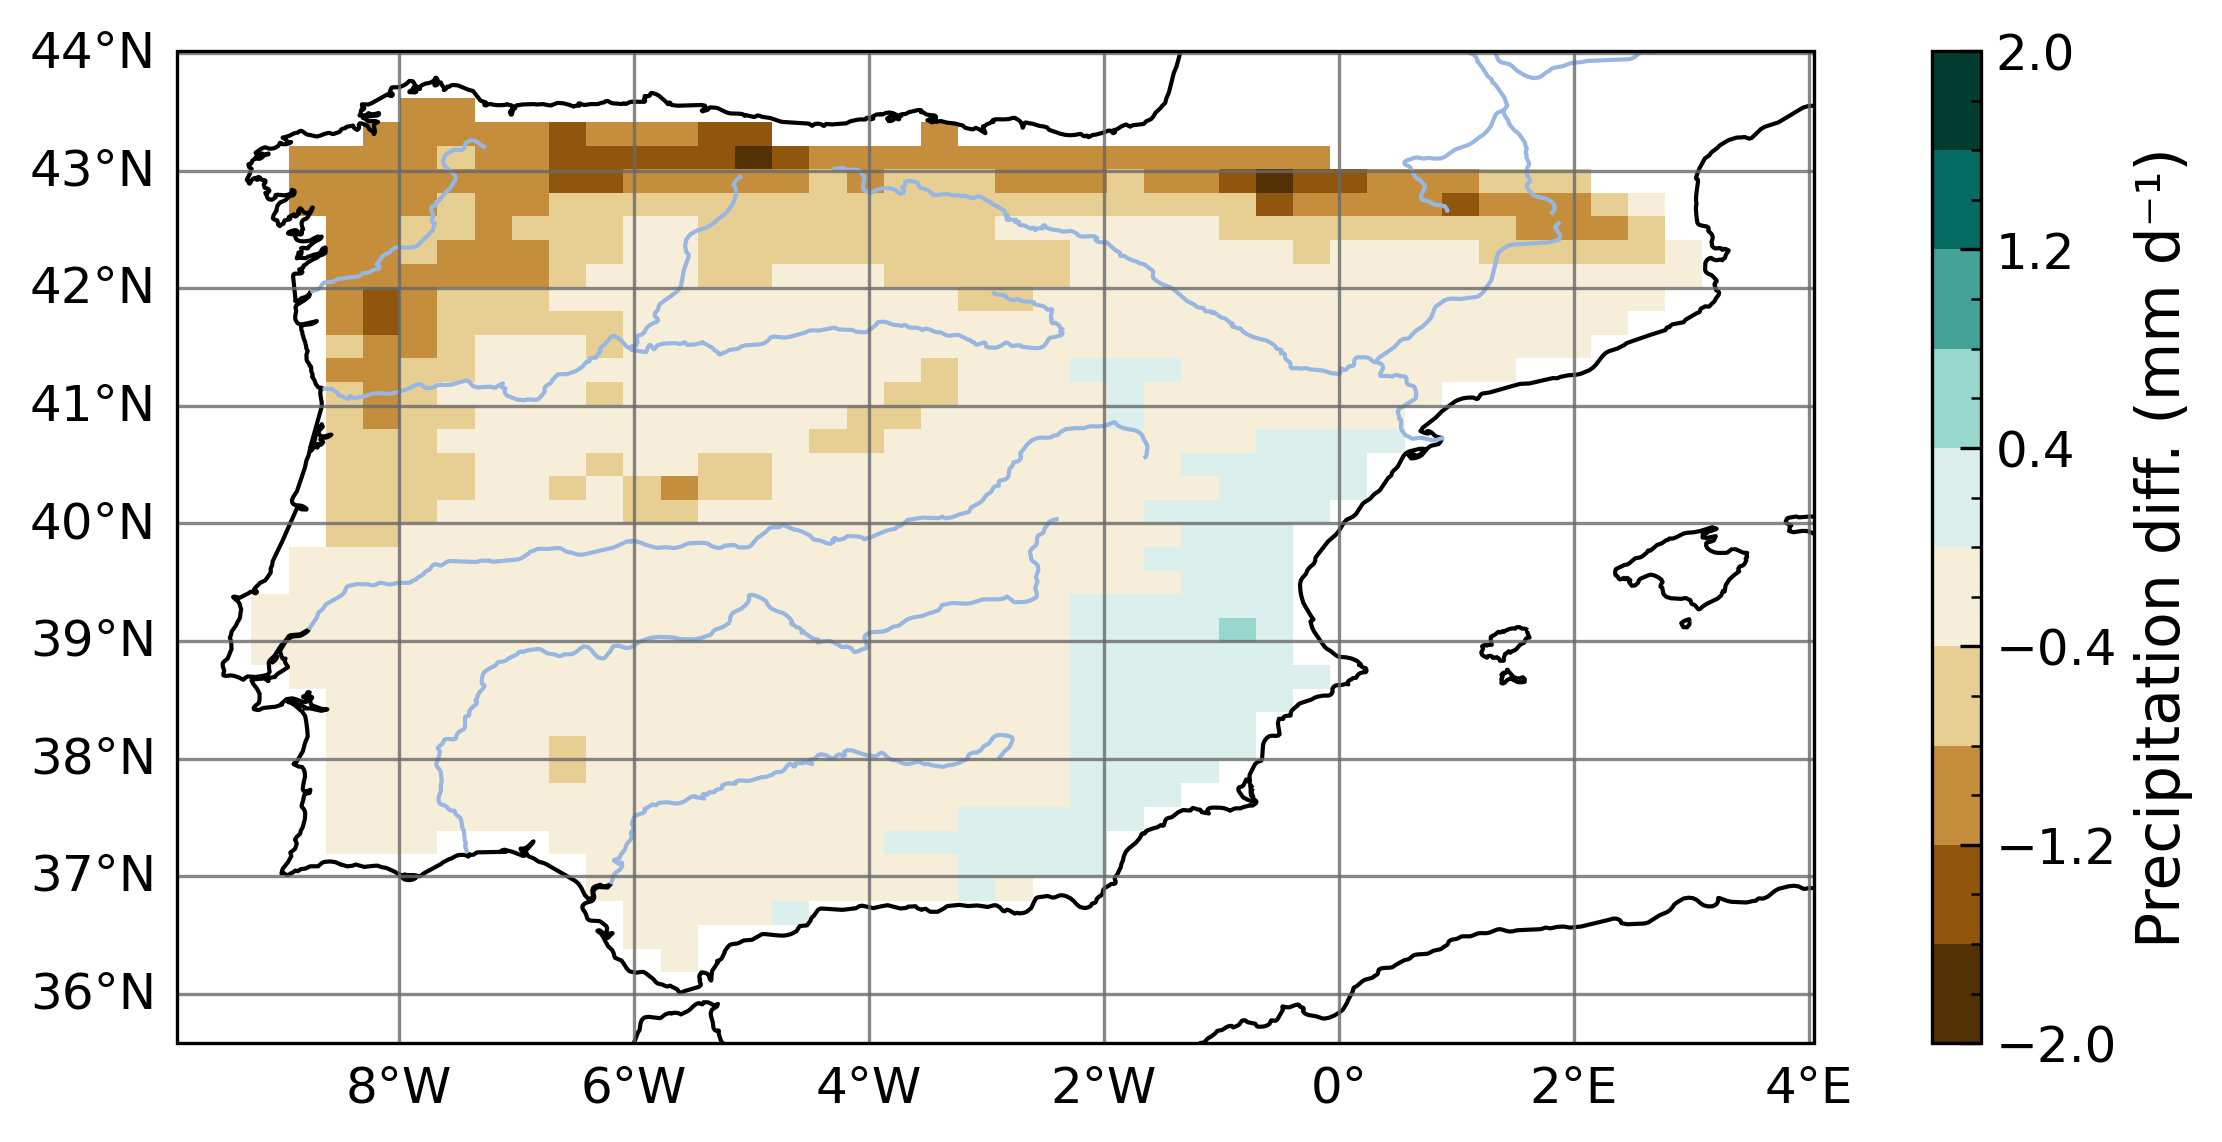
\includegraphics[width=\textwidth]{images/chap4/future/diffmap_precip_presfut.png}
        \end{subfigure} &
        %evap
        \begin{subfigure}[b]{0.5\textwidth}
            \caption{ET difference}
            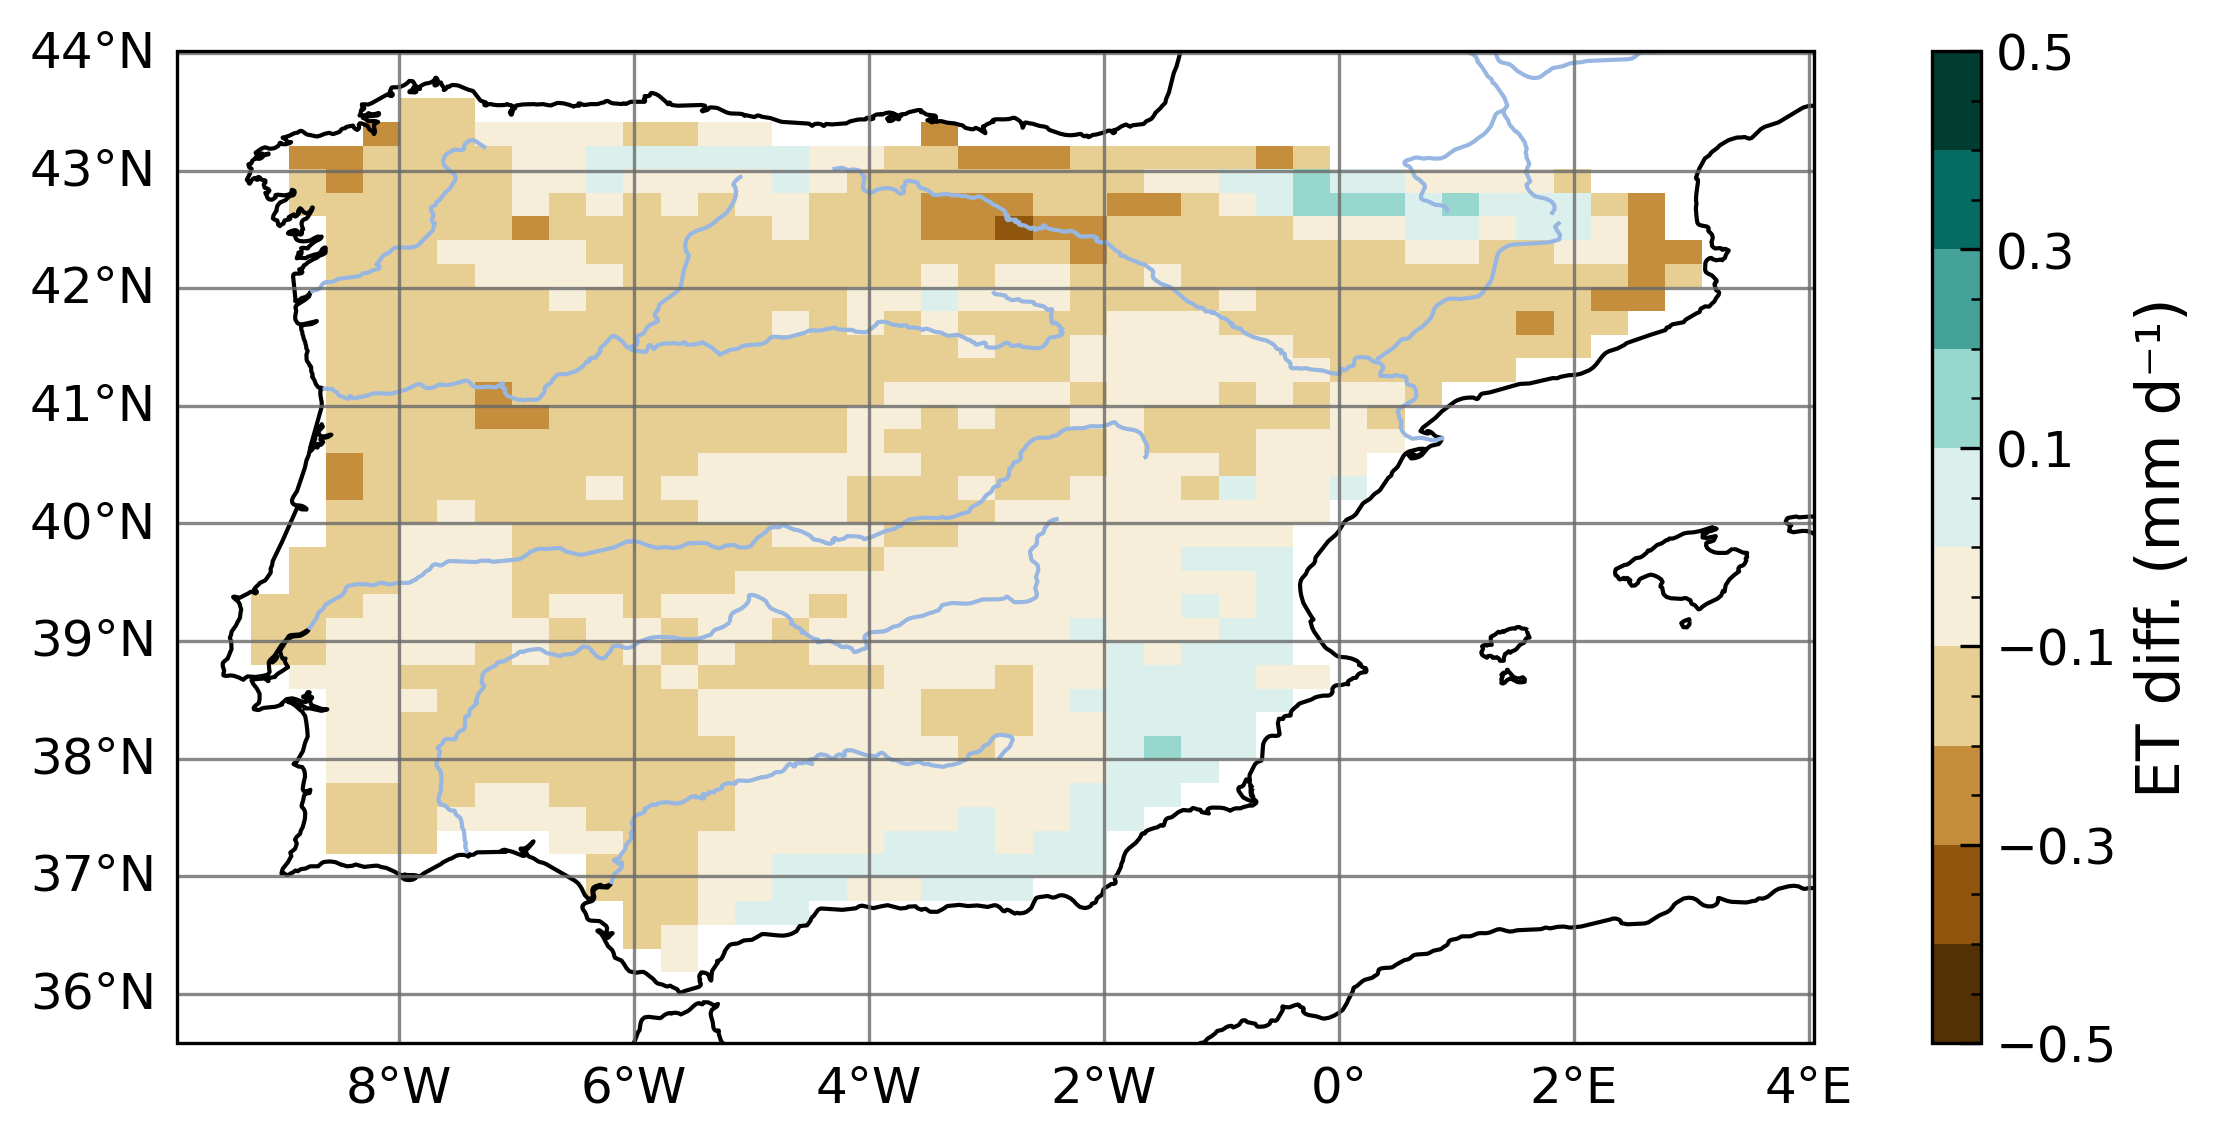
\includegraphics[width=\textwidth]{images/chap4/future/diffmap_evap_presfut.png}
        \end{subfigure} \\


        %q2m
        \begin{subfigure}[b]{0.5\textwidth}
            \caption{2-m specific humidity difference}
            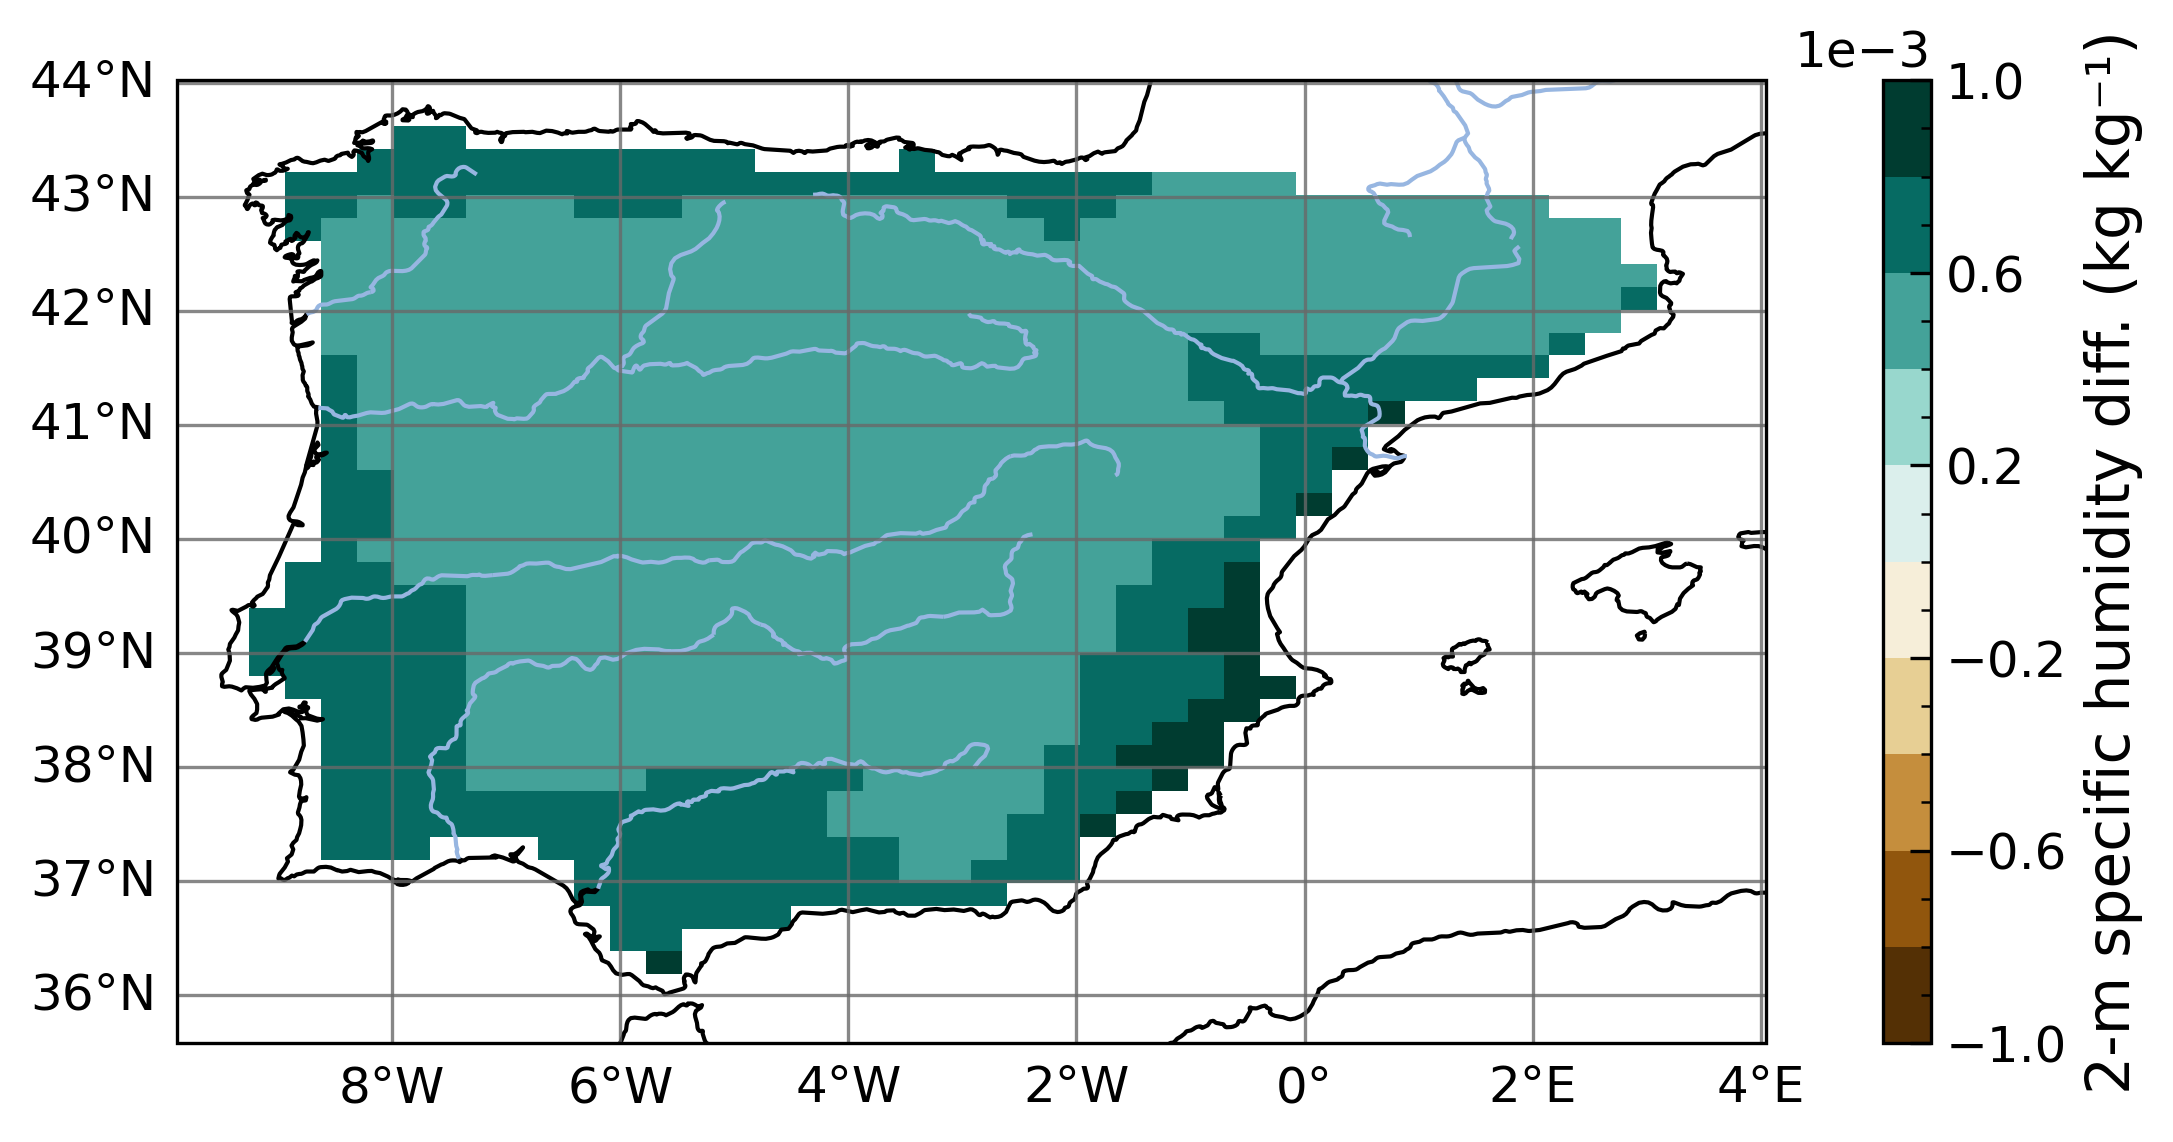
\includegraphics[width=\textwidth]{images/chap4/future/diffmap_q2m_presfut.png}
        \end{subfigure} &
        %rh2m
        \begin{subfigure}[b]{0.5\textwidth}
            \caption{2-m relative humidity difference}
            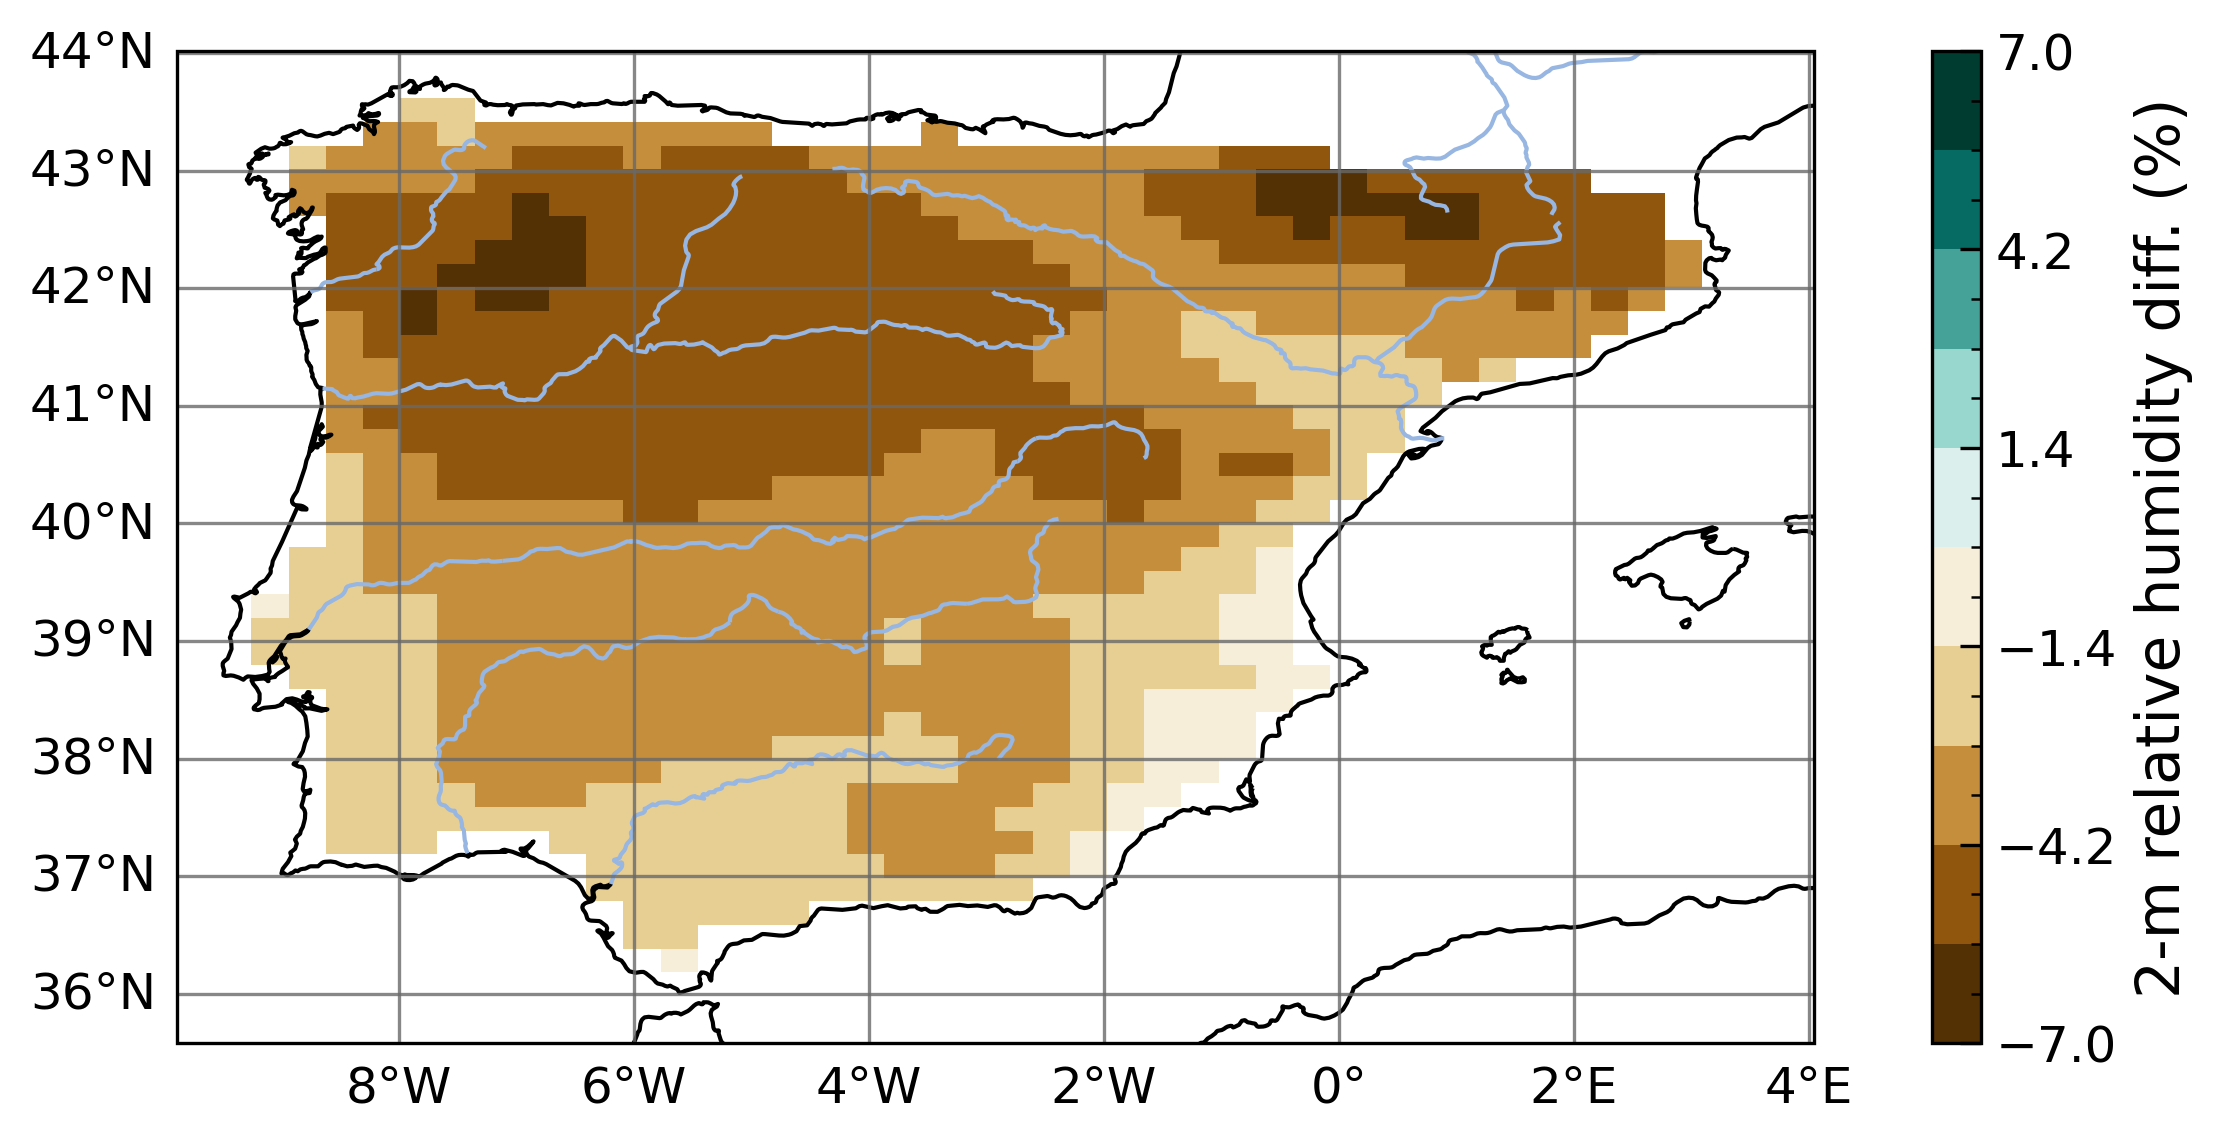
\includegraphics[width=\textwidth]{images/chap4/future/diffmap_rh2m_presfut.png}
        \end{subfigure} \\

        %SWdnSFC
        \begin{subfigure}[b]{0.5\textwidth}
            \caption{Downwelling shortwave radiation difference}
            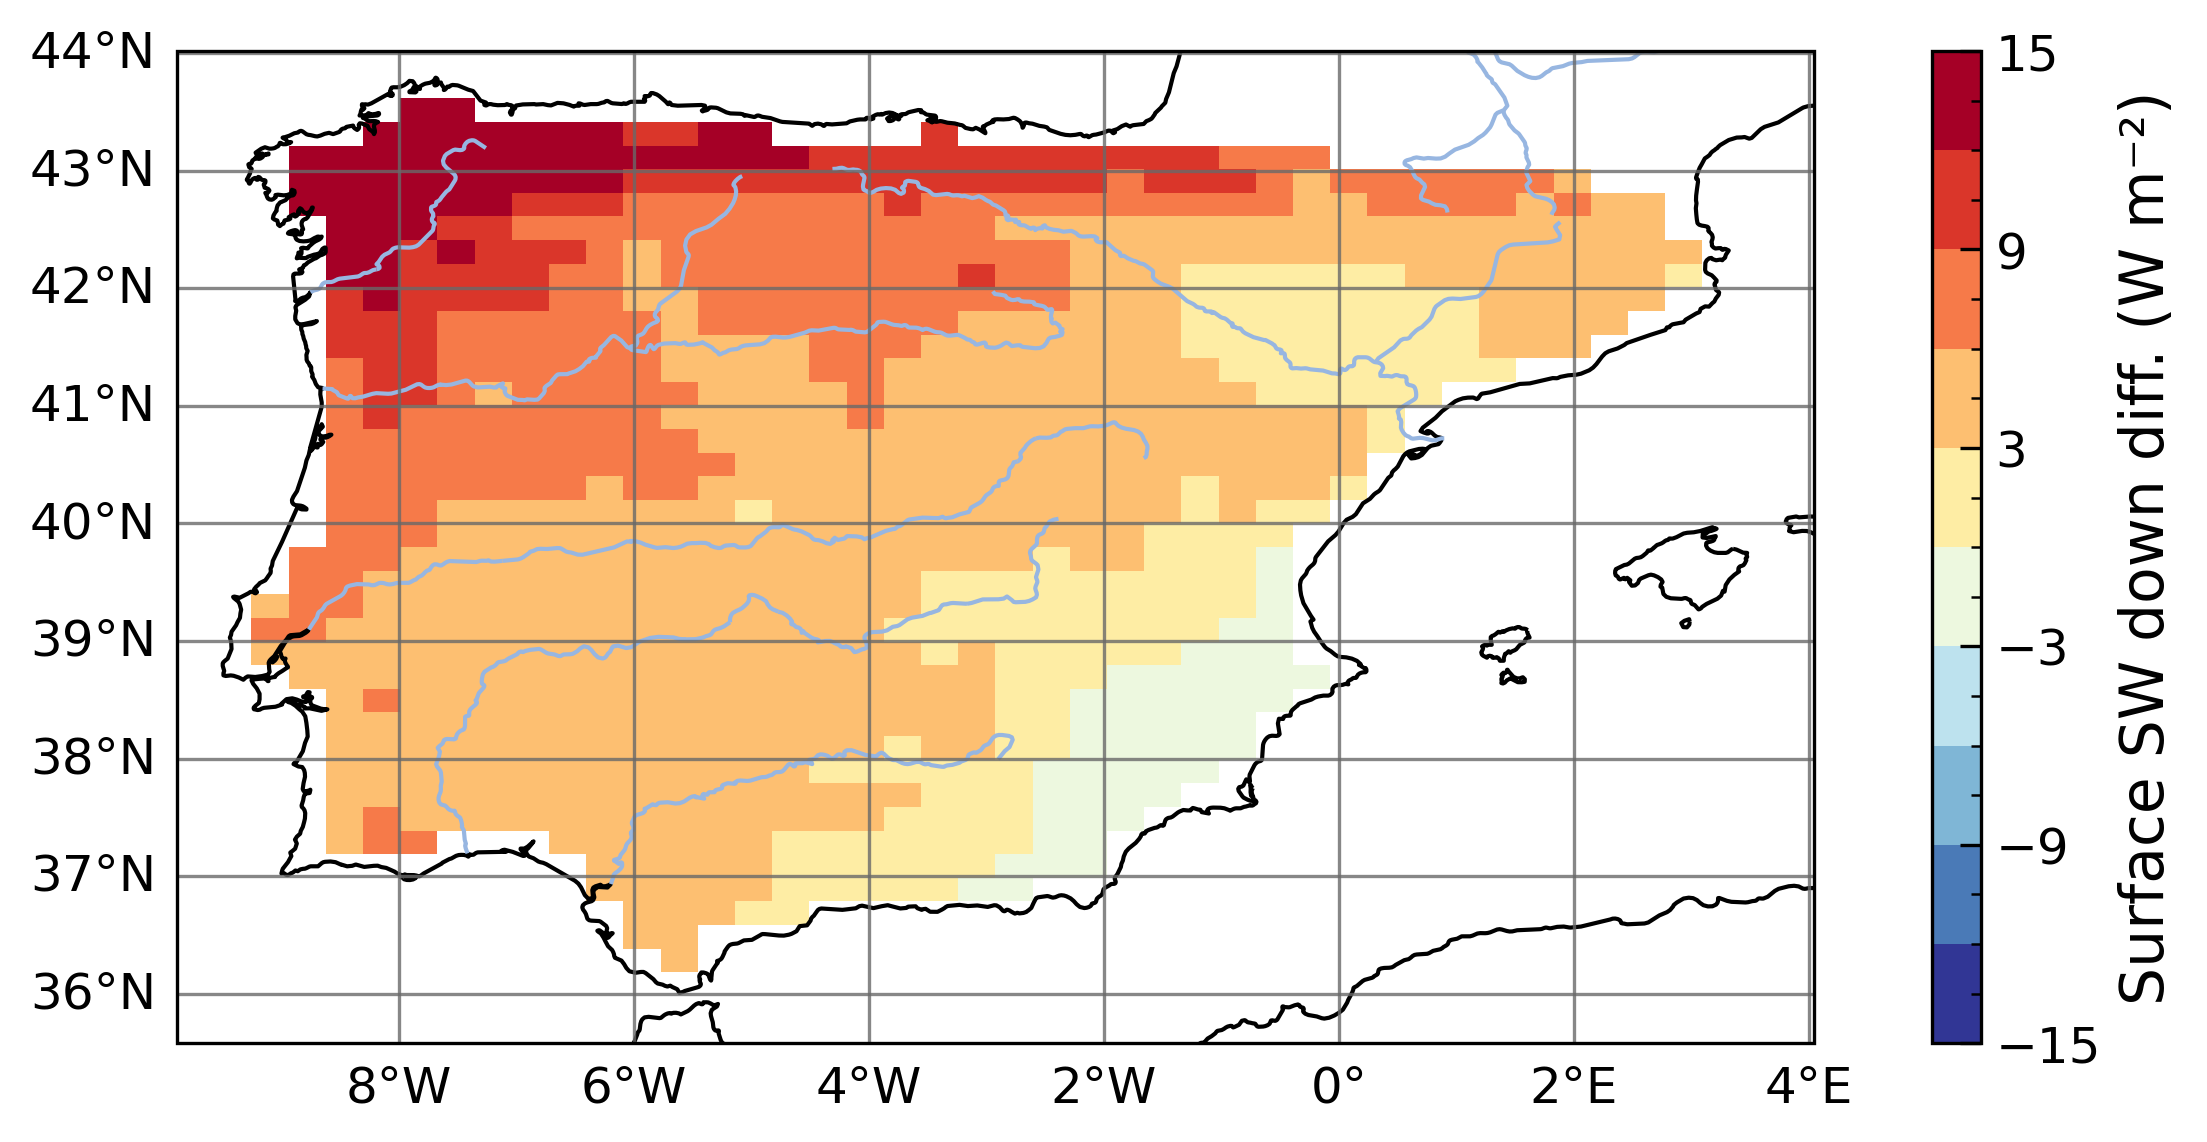
\includegraphics[width=\textwidth]{images/chap4/future/diffmap_SWdnSFC_presfut.png}
        \end{subfigure} &
        %LWdnSFC
        \begin{subfigure}[b]{0.5\textwidth}
            \caption{Downwelling longwave radiation difference}
            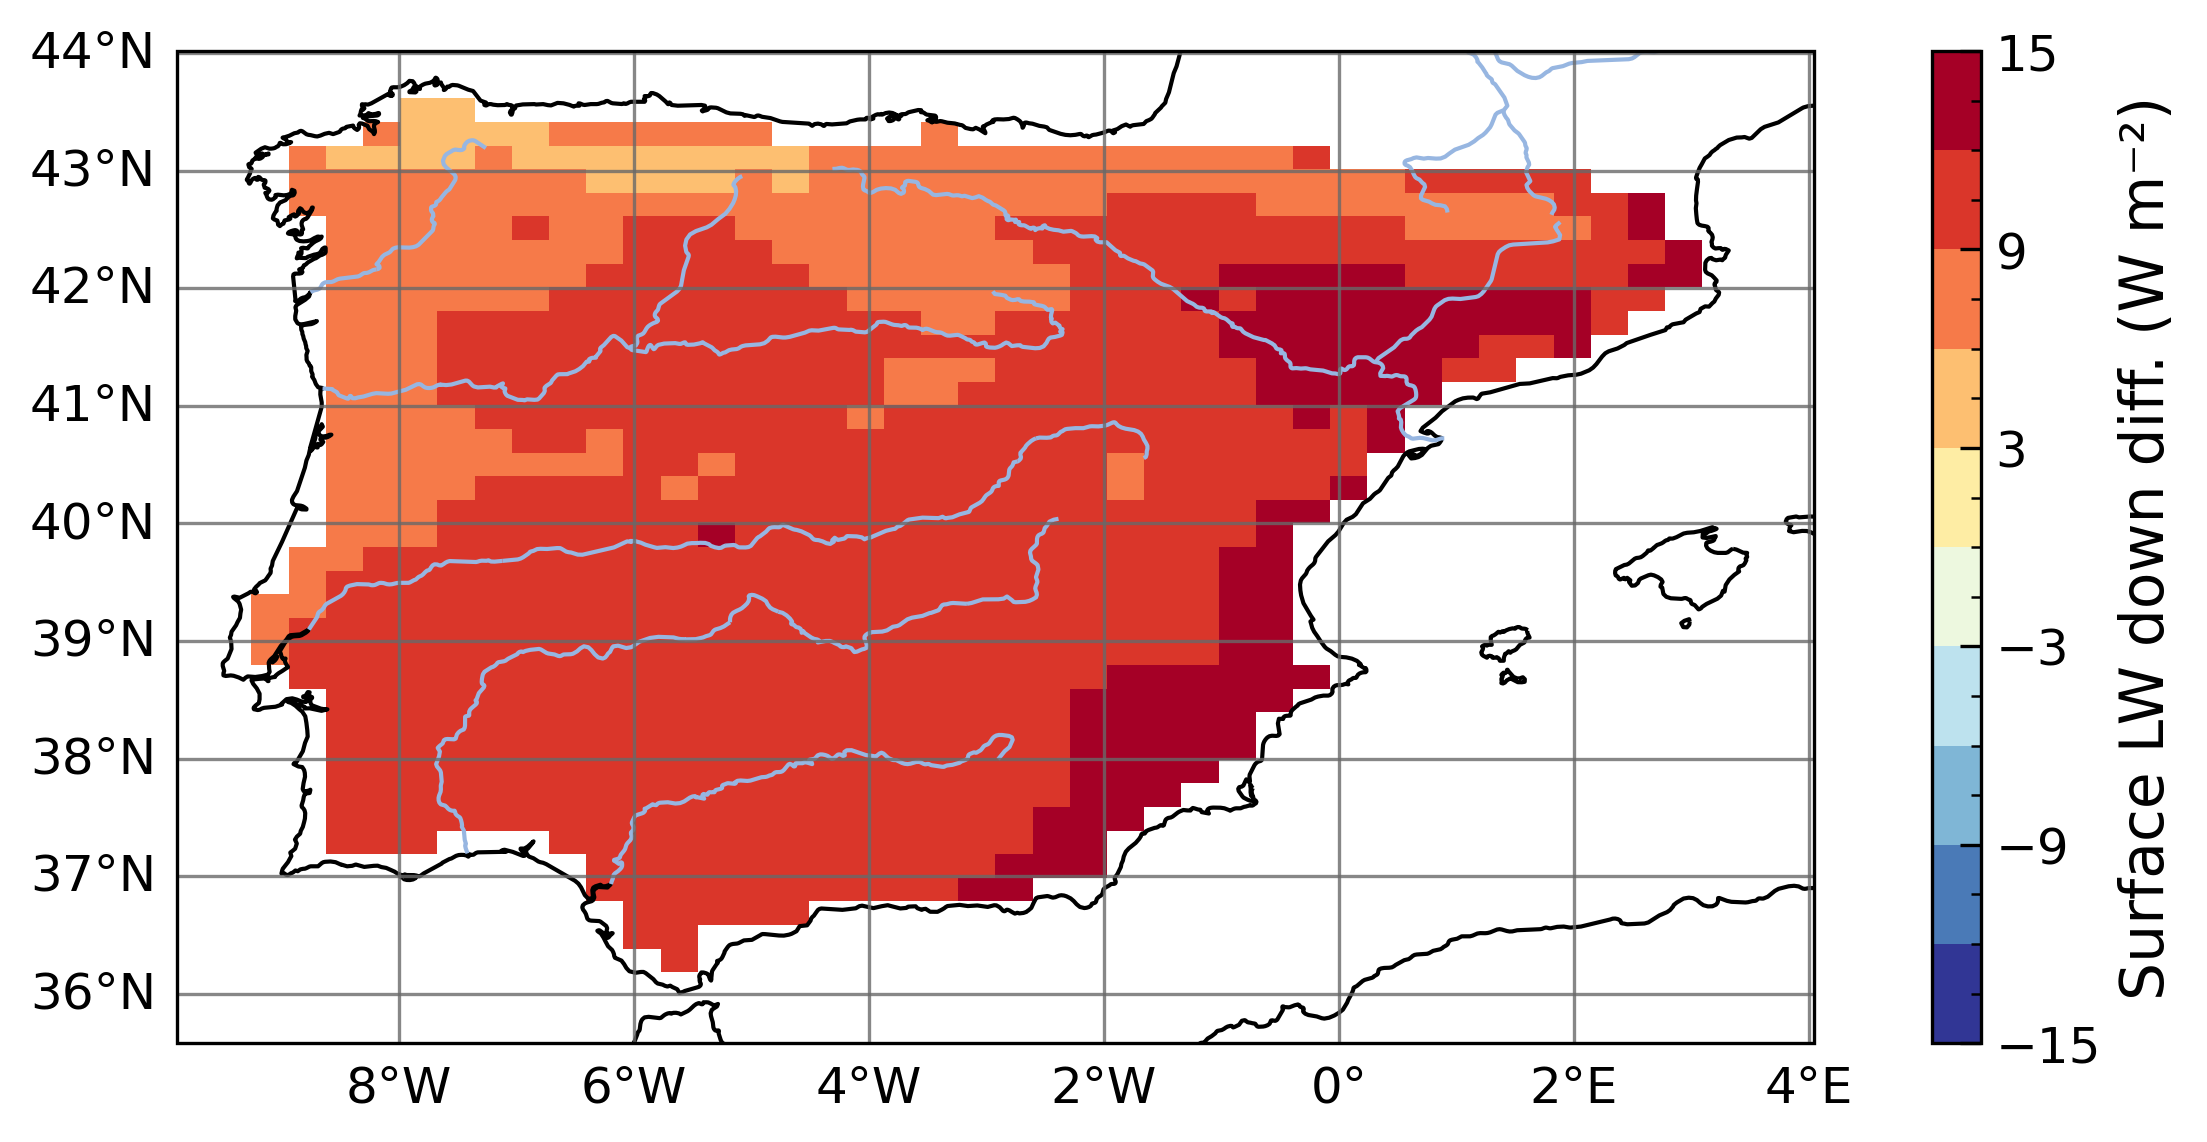
\includegraphics[width=\textwidth]{images/chap4/future/diffmap_LWdnSFC_presfut.png}
        \end{subfigure} \\

        % %pblh
        % \begin{subfigure}[b]{0.5\textwidth}
        %     \caption{}
        %     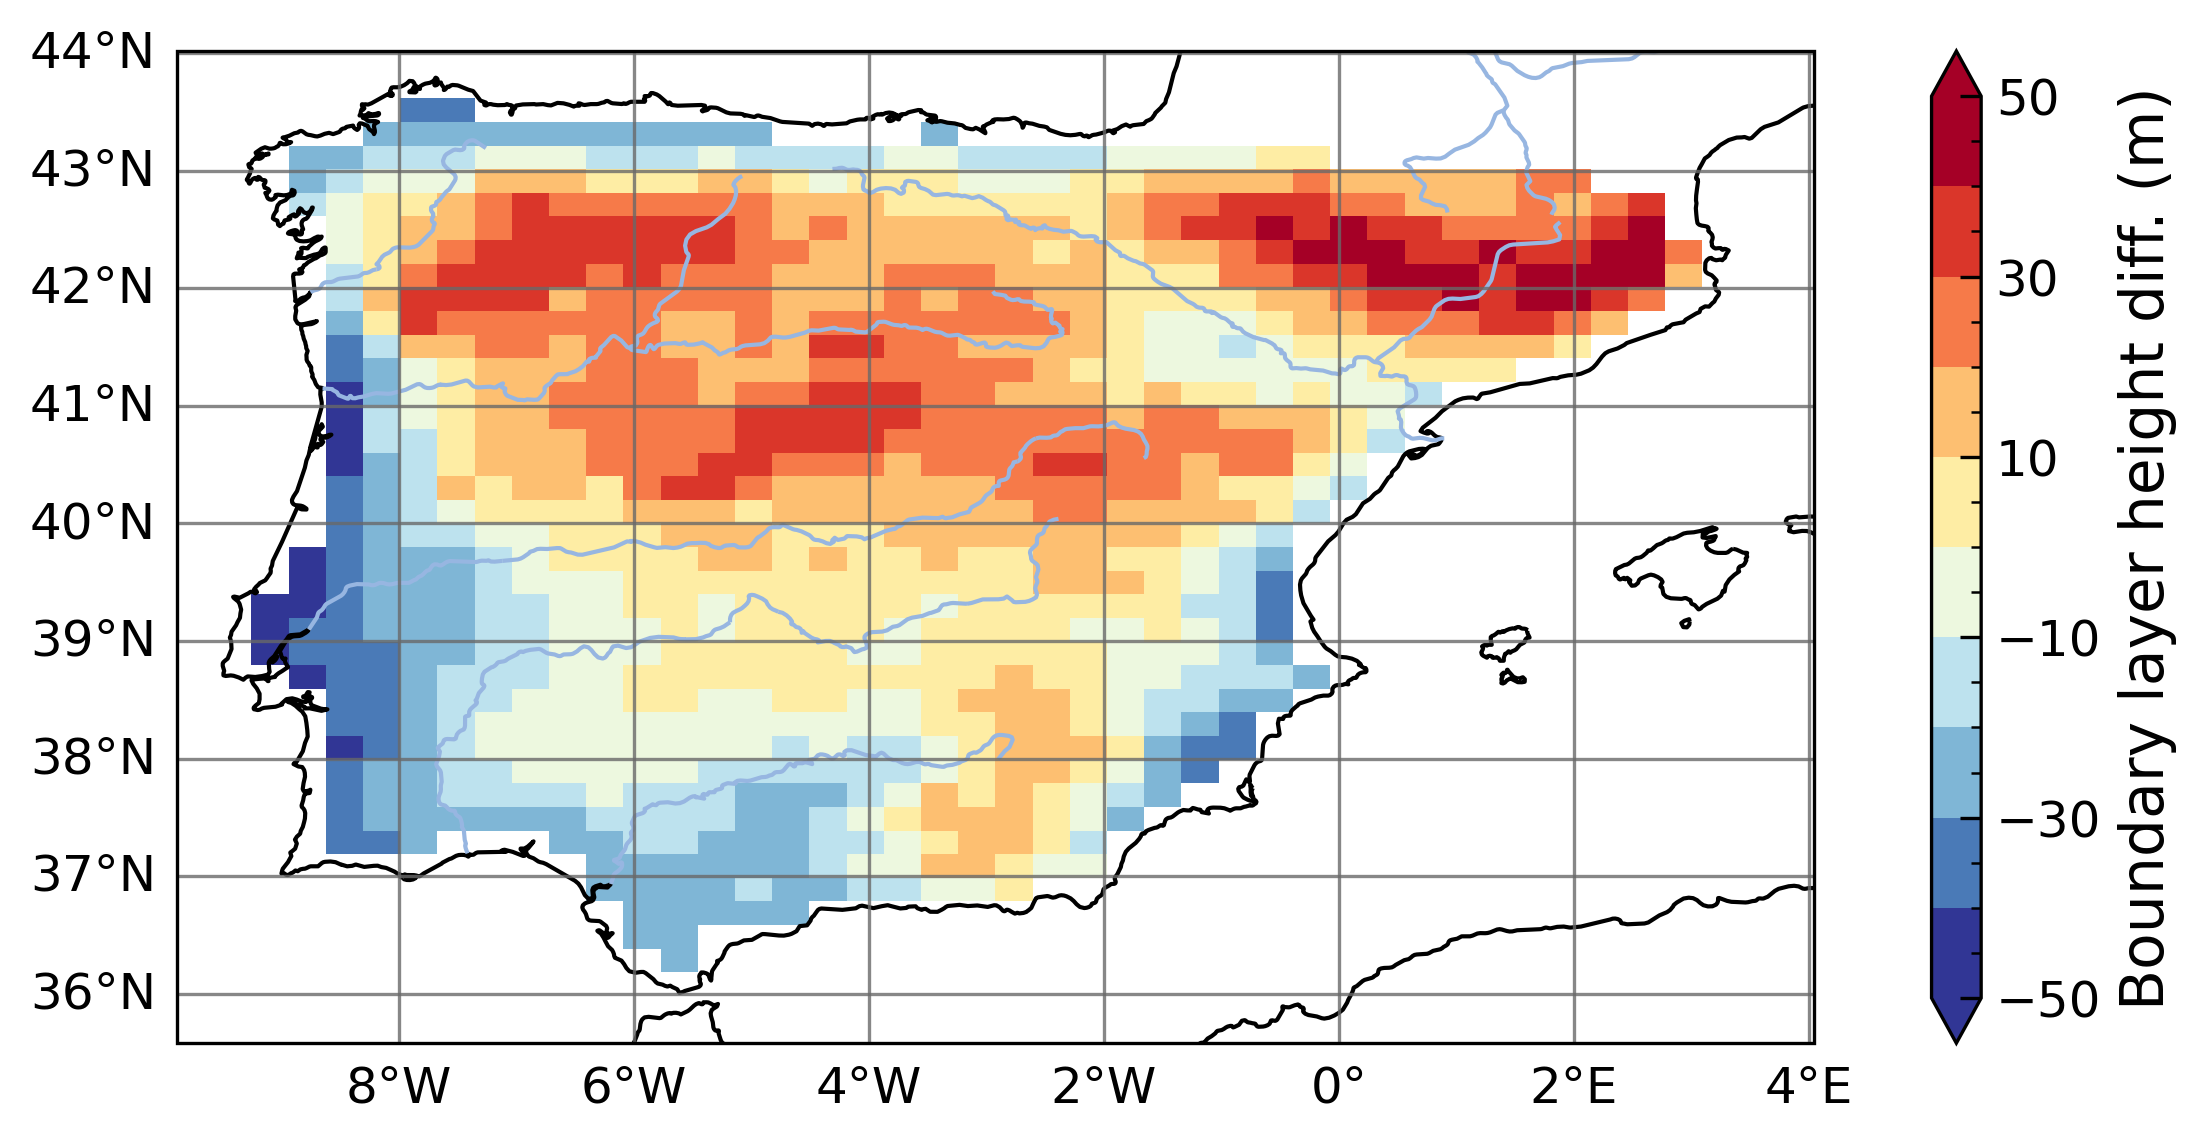
\includegraphics[width=\textwidth]{images/chap4/future/diffmap_s_pblh_presfut.png}
        % \end{subfigure} &
        % %lcl
        % \begin{subfigure}[b]{0.5\textwidth}
        %     \caption{}
        %     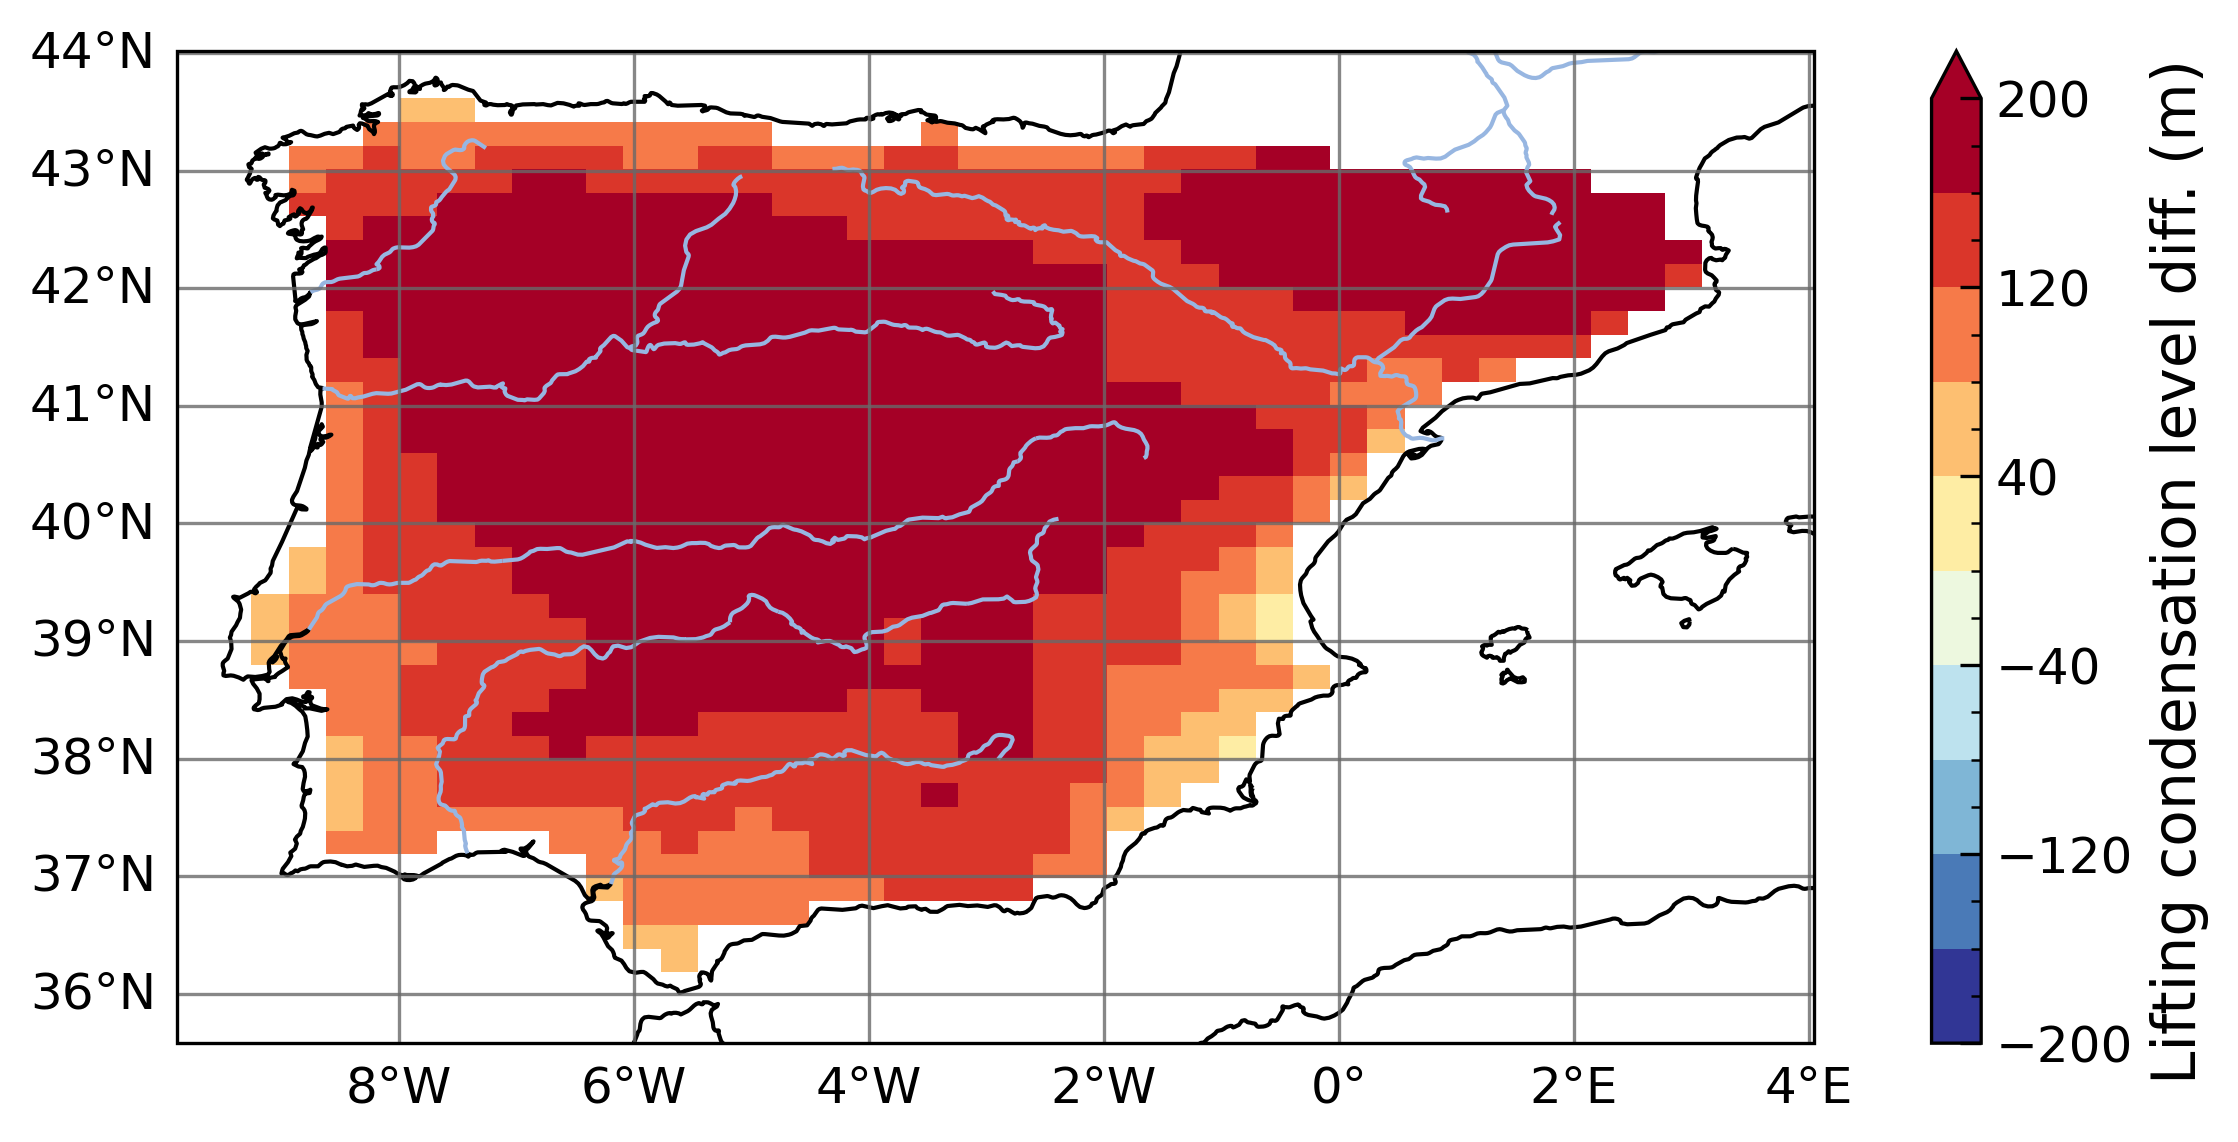
\includegraphics[width=\textwidth]{images/chap4/future/diffmap_s_lcl_presfut.png}
        % \end{subfigure} \\
    \end{tabular}
    \caption{Impacts of climate change over the Iberian Peninsula. Annual mean difference between \futnoirr (2050-2062) and  \presnoirr (2010-2022).}
    \label{fig:diffmaps_present_future}
\end{figure}

\clearpage

\subsection{Impacts of irrigation under climate change}

%figure : map and SC of irrigation in the future
\begin{figure}[htbp]
    \centering
    \begin{tabular}{cc}
        %precip
        \begin{subfigure}[b]{0.48\textwidth}
            \caption{Irrigation annual mean}
            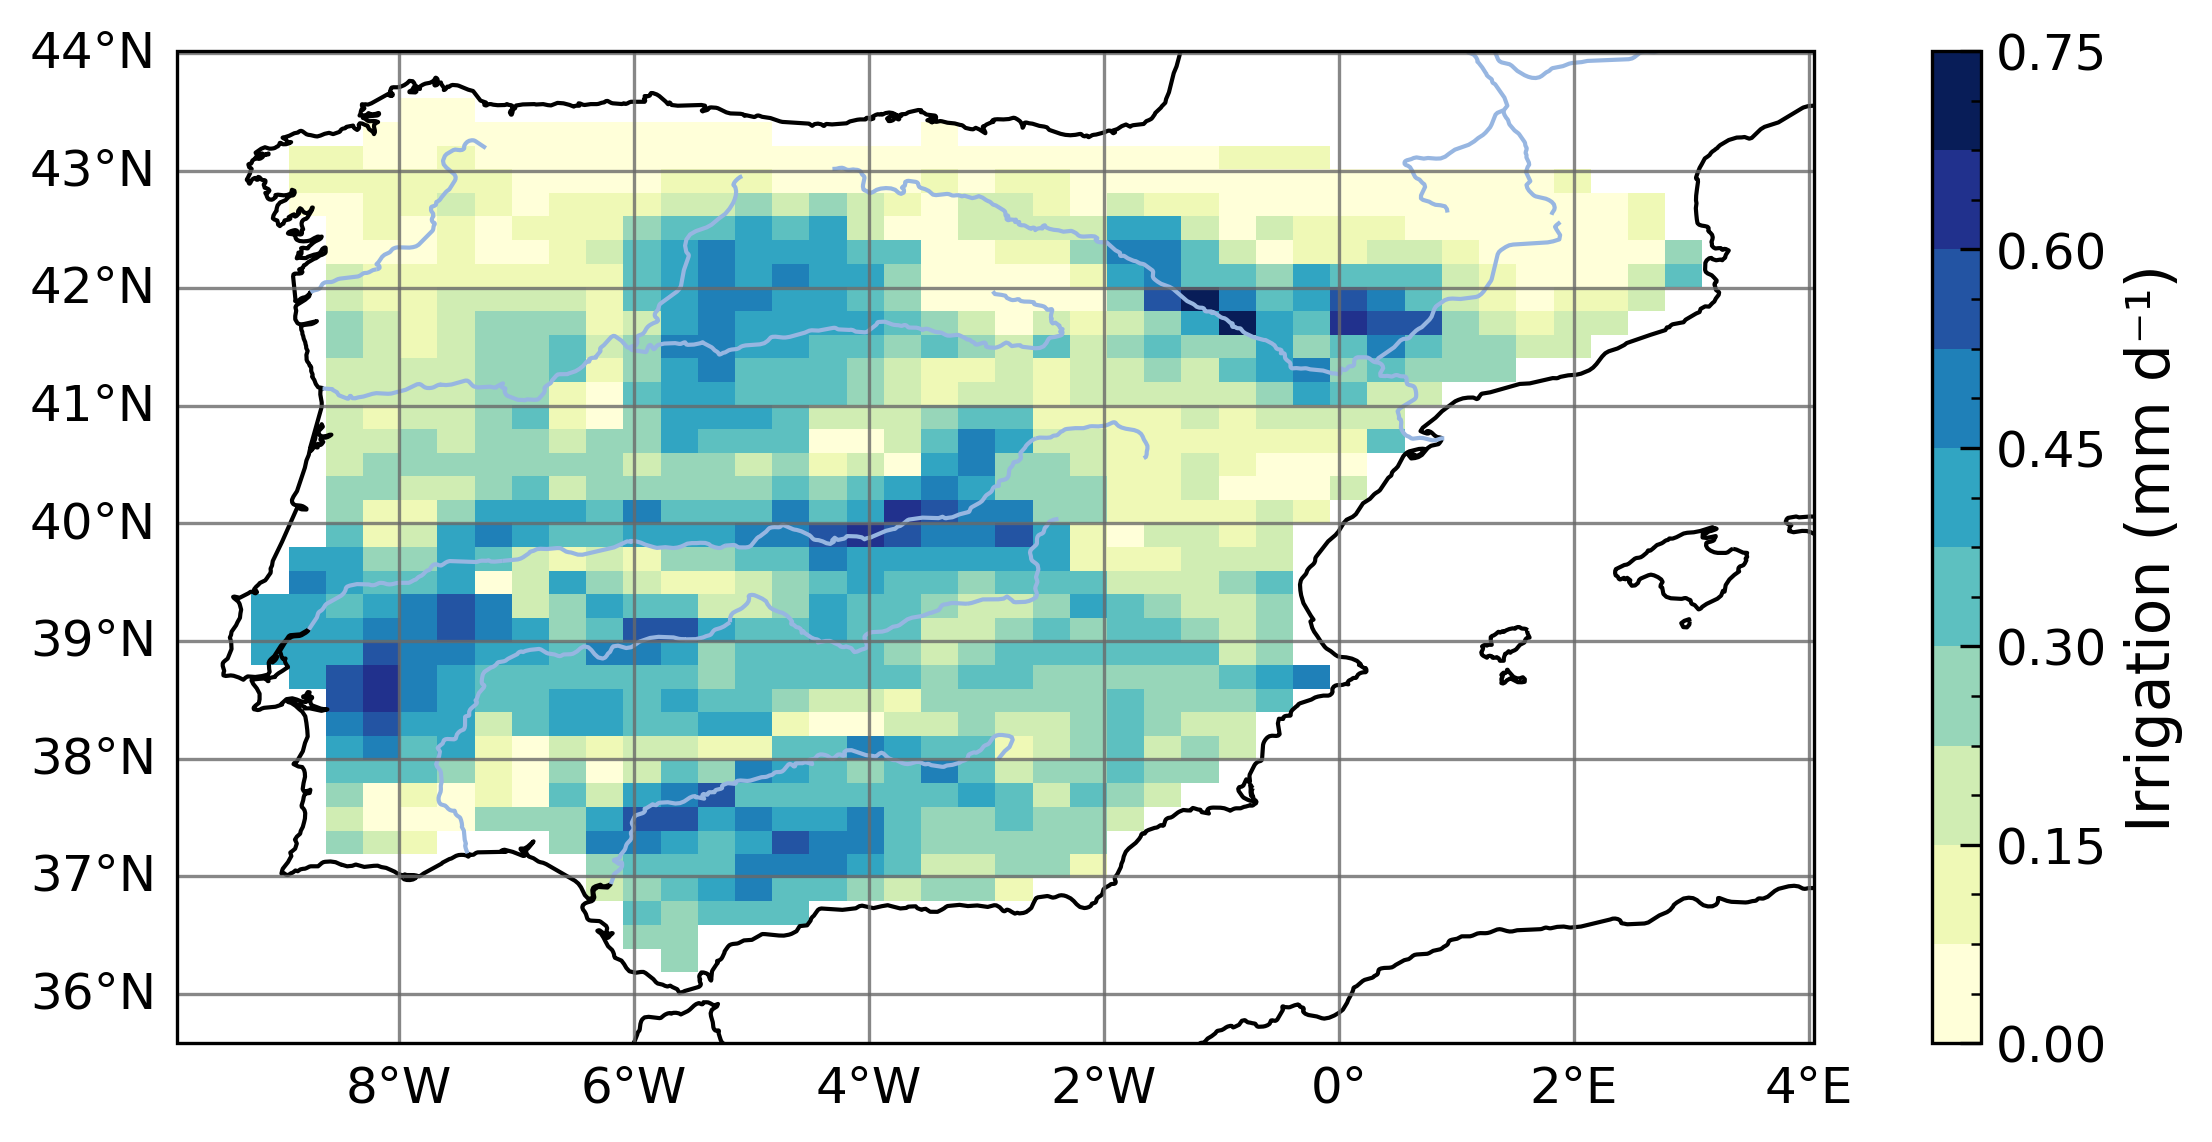
\includegraphics[width=\textwidth]{images/chap4/future/map_irrigation_fut.png}
        \end{subfigure} &
        \begin{subfigure}[b]{0.46\textwidth}
            \caption{Irrigation mean seasonal cycle}
            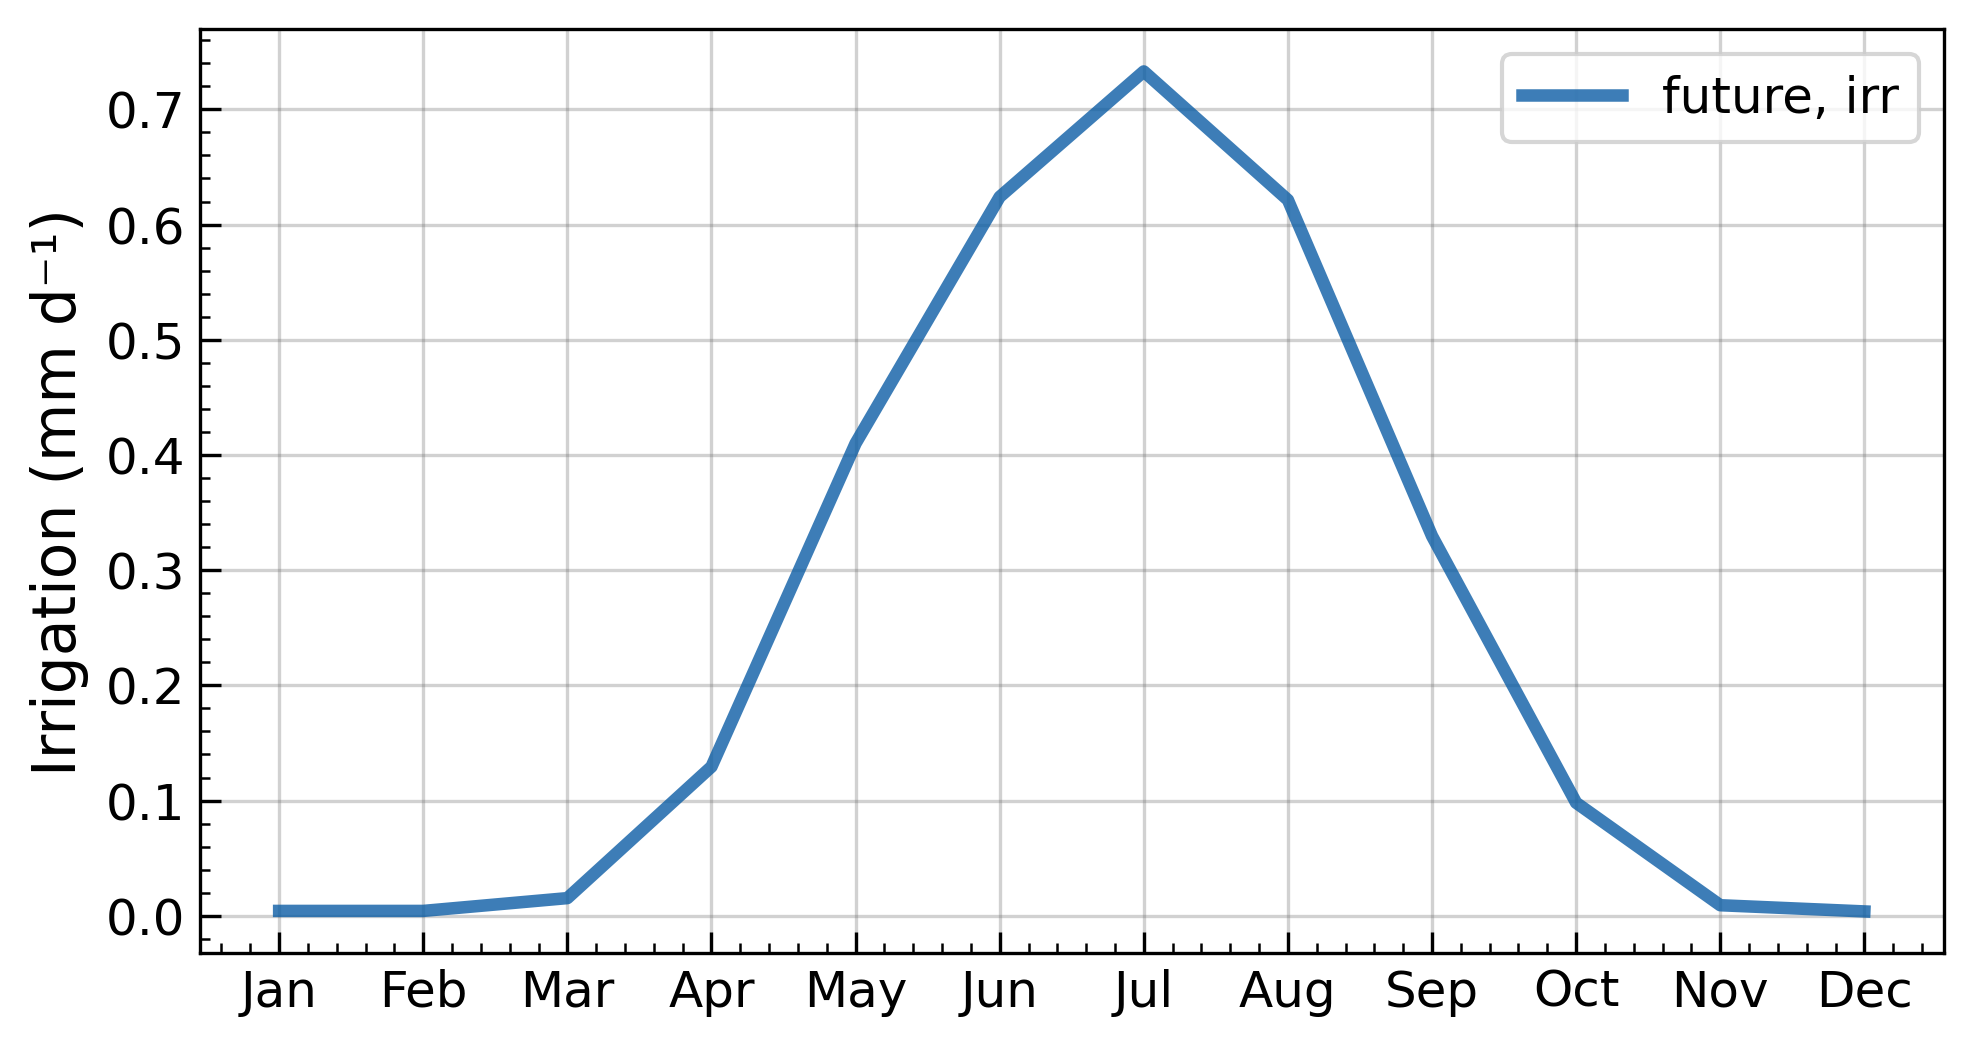
\includegraphics[width=\textwidth]{images/chap4/future/SC_irrigation_fut.png}
        \end{subfigure}
    \end{tabular}
    \caption{Annual mean and seasonal cycle of irrigation over the Iberian Peninsula in the \futirr simulation (2050-2062).}
    \label{fig:future_irrig}
\end{figure}

Irrigation in the \futirr simulation is largest in the valleys of the Ebro, Douro, Tagus, Guadiana and Guadalquivir rivers (Fig. \ref{fig:future_irrig}a). Due to modelling choices, it is near-zero in winter, and follows a rather symmetrical seasonal cycle from spring to autumn, with a peak in July (Fig. \ref{fig:future_irrig}b).
%option: direct comparison with simulated irrigation in present ? Tricky : one big difference is the forcing used (ERA5 vs ICOLMDZOR) ; another is the fact that for this simulation, routing was inappropriately paramterized, leading to huge volumes in reservoirs... (new simulation with same parameters ongoing...)

%turbulent fluxes
Its most direct atmospheric impact is an increase in ET of similar amplitude to the irrigation amounts (Fig. \ref{fig:diffmaps_future_irr}d), which largely compensates for the decrease in ET induced by climate change. This increase of the latent heat flux is directly linked to a decrease of the sensible heat flux (Fig. \ref{fig:diffmaps_future_irr}b) reaching -15 W \persqm in the most irrigated valleys. 
%t2m
This new partitionning of surface energy leads to a cooler air over most of the domain (Fig. \ref{fig:diffmaps_future_irr}a). The largest decreases occur  over the intensely irrigated areas where 2-m temperature is lowered by 0.5°C on annual average and 1°C in summer. %todo:appendix figure or remove ?
Contrary to ET, this consequence of irrigation is insufficient to compensate the impact of climate change, which induces 2-m temperature increases of 2°C annually and larger than 3°C in summer. %todo:appendix figure or remove ?
%q2m RH2m
Regarding humidity, \futirr is moister than \futnoirr (Fig. \ref{fig:diffmaps_future_irr}e) but some intensely irrigated areas such as the Ebro valley show smaller increases in specific humidity than others, suggesting a stronger mixing of the lower atmosphere in these regions. Combined with the changes in temperature, the increase of specific humidity also leads to an increase in relative humidity  (Fig. \ref{fig:diffmaps_future_irr}f), wich opposes the impact of climate change.
%ABL
The structure of the boundary layer is also affected by irrigation. Stabilization dominates and follows the same pattern as irrigation, as a consequence of cooling and of the reduced sensible heat flux. The ABL height is lowered by more than a 100m in the most intensely irrigated grid areas. 
Due to the moistening and cooling of the atmosphere, the lifting condensation level is also lowered. Similarly to the changes in 2-m humidity, LCL is more affected in the Tagus, Guadiana and Guadalquivir basins than in the Ebro and Douro basins.
As explained in Section \ref{sec:article1}, the lowering of both the ABL height and LCL point to to opposite effects on cloud formation and precipitation, since one reflects a more stable atmosphere less likely to form clouds through convection, while the other is associated with a moister and cooler atmosphere where condensation is more likely. As a consequence, the impact of irrigation on precipitation is rather limited and the only significant structures that emerge are precipitation increases in the highest moutain ranges, the Iberian System and the Pyrenees.

%figure : diff maps (future, irr - no_irr)
\begin{figure}[htbp]
    \centering
    \begin{tabular}{cc}
        %t2m
        \begin{subfigure}[b]{0.5\textwidth}
            \caption{2-m temperature difference}
            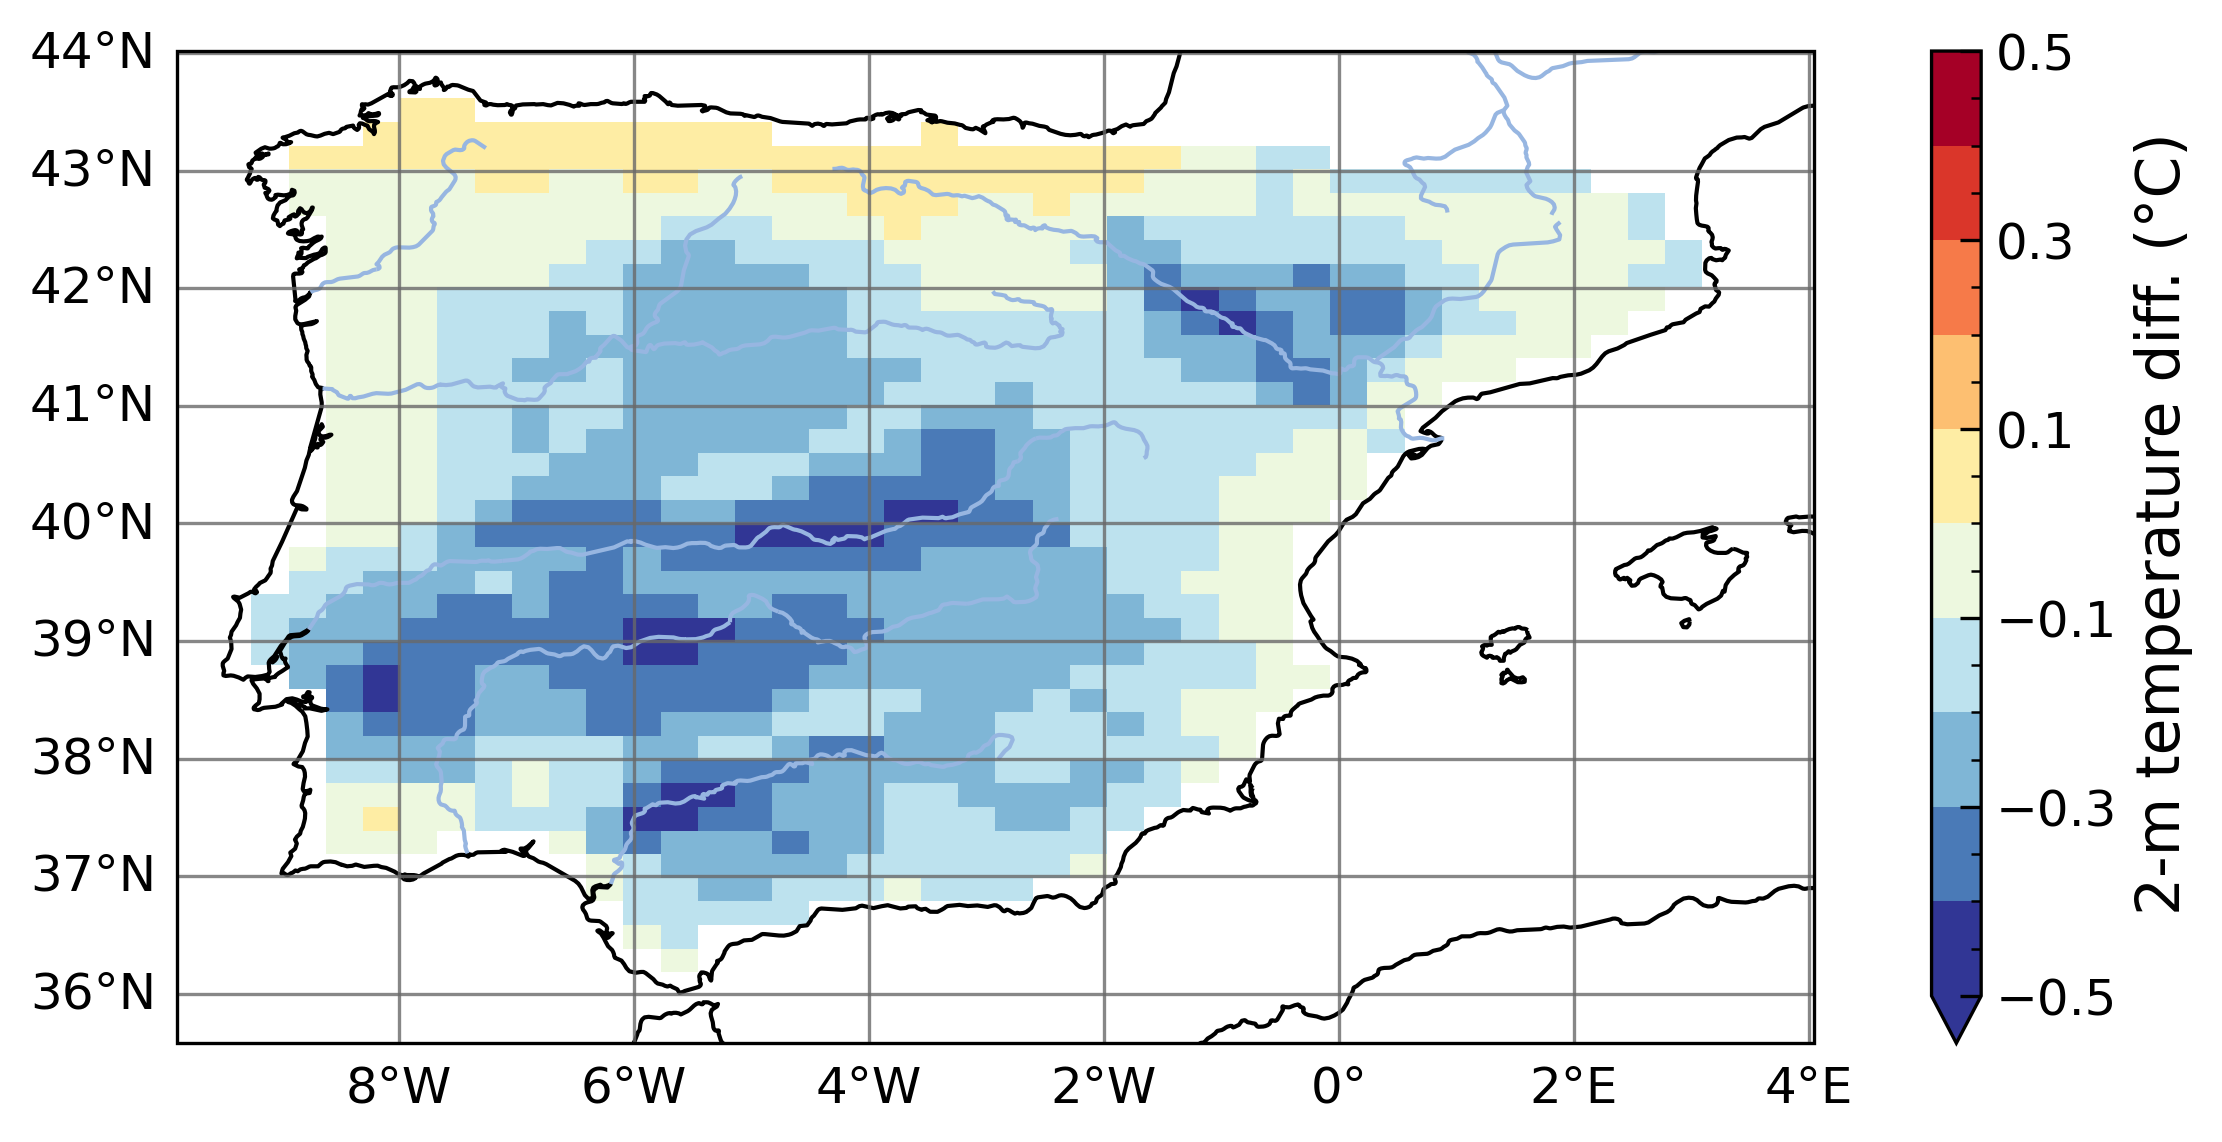
\includegraphics[width=\textwidth]{images/chap4/future/diffmap_t2m_futirr.png}
        \end{subfigure} &
        %fluxsens
        \begin{subfigure}[b]{0.5\textwidth}
            \caption{Sensible heat flux difference}
            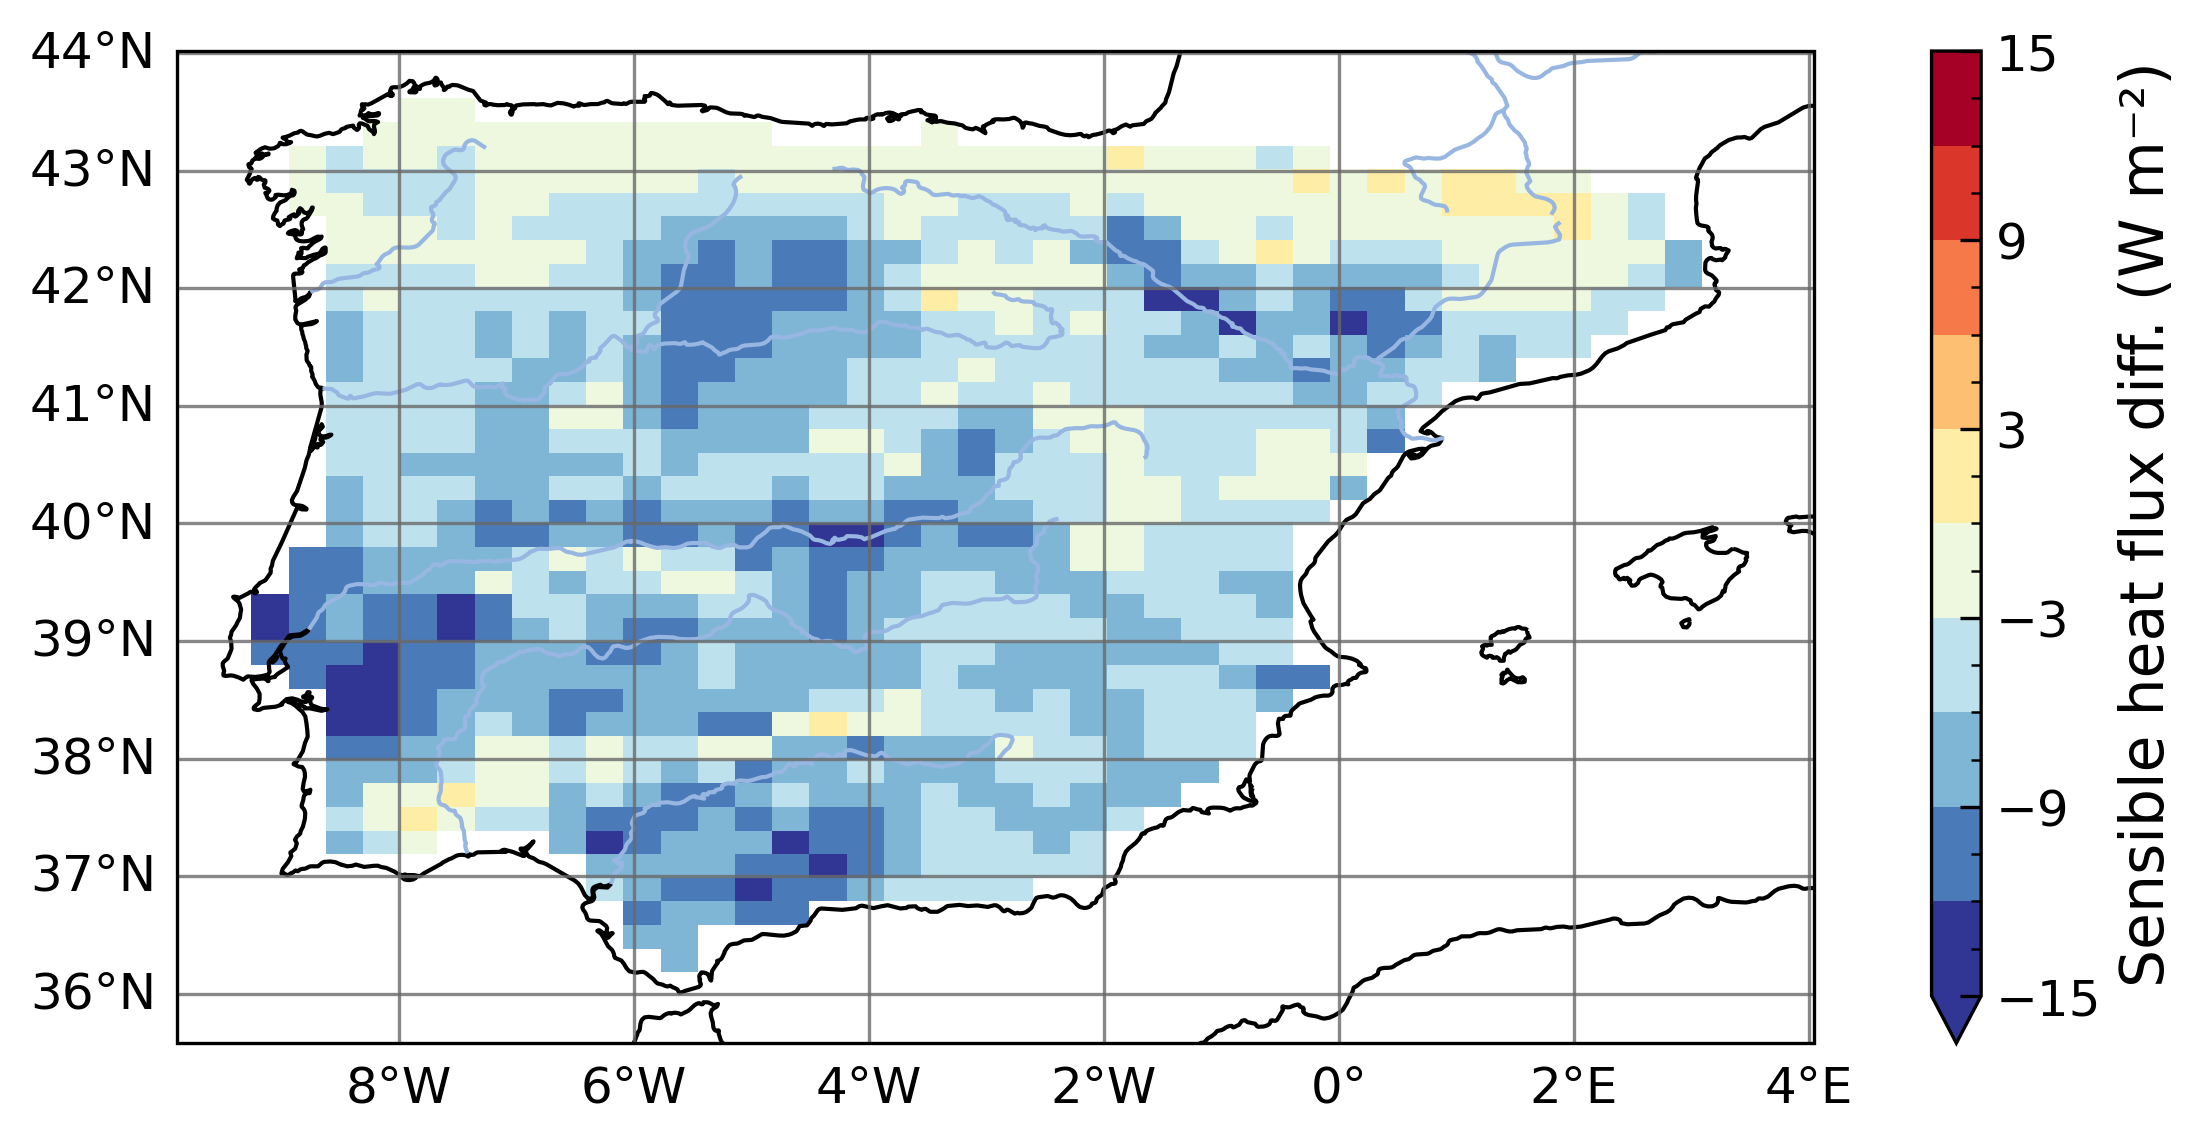
\includegraphics[width=\textwidth]{images/chap4/future/diffmap_fluxsens_futirr.png}
        \end{subfigure} \\

        %precip
        \begin{subfigure}[b]{0.5\textwidth}
            \caption{Precipitation difference}
            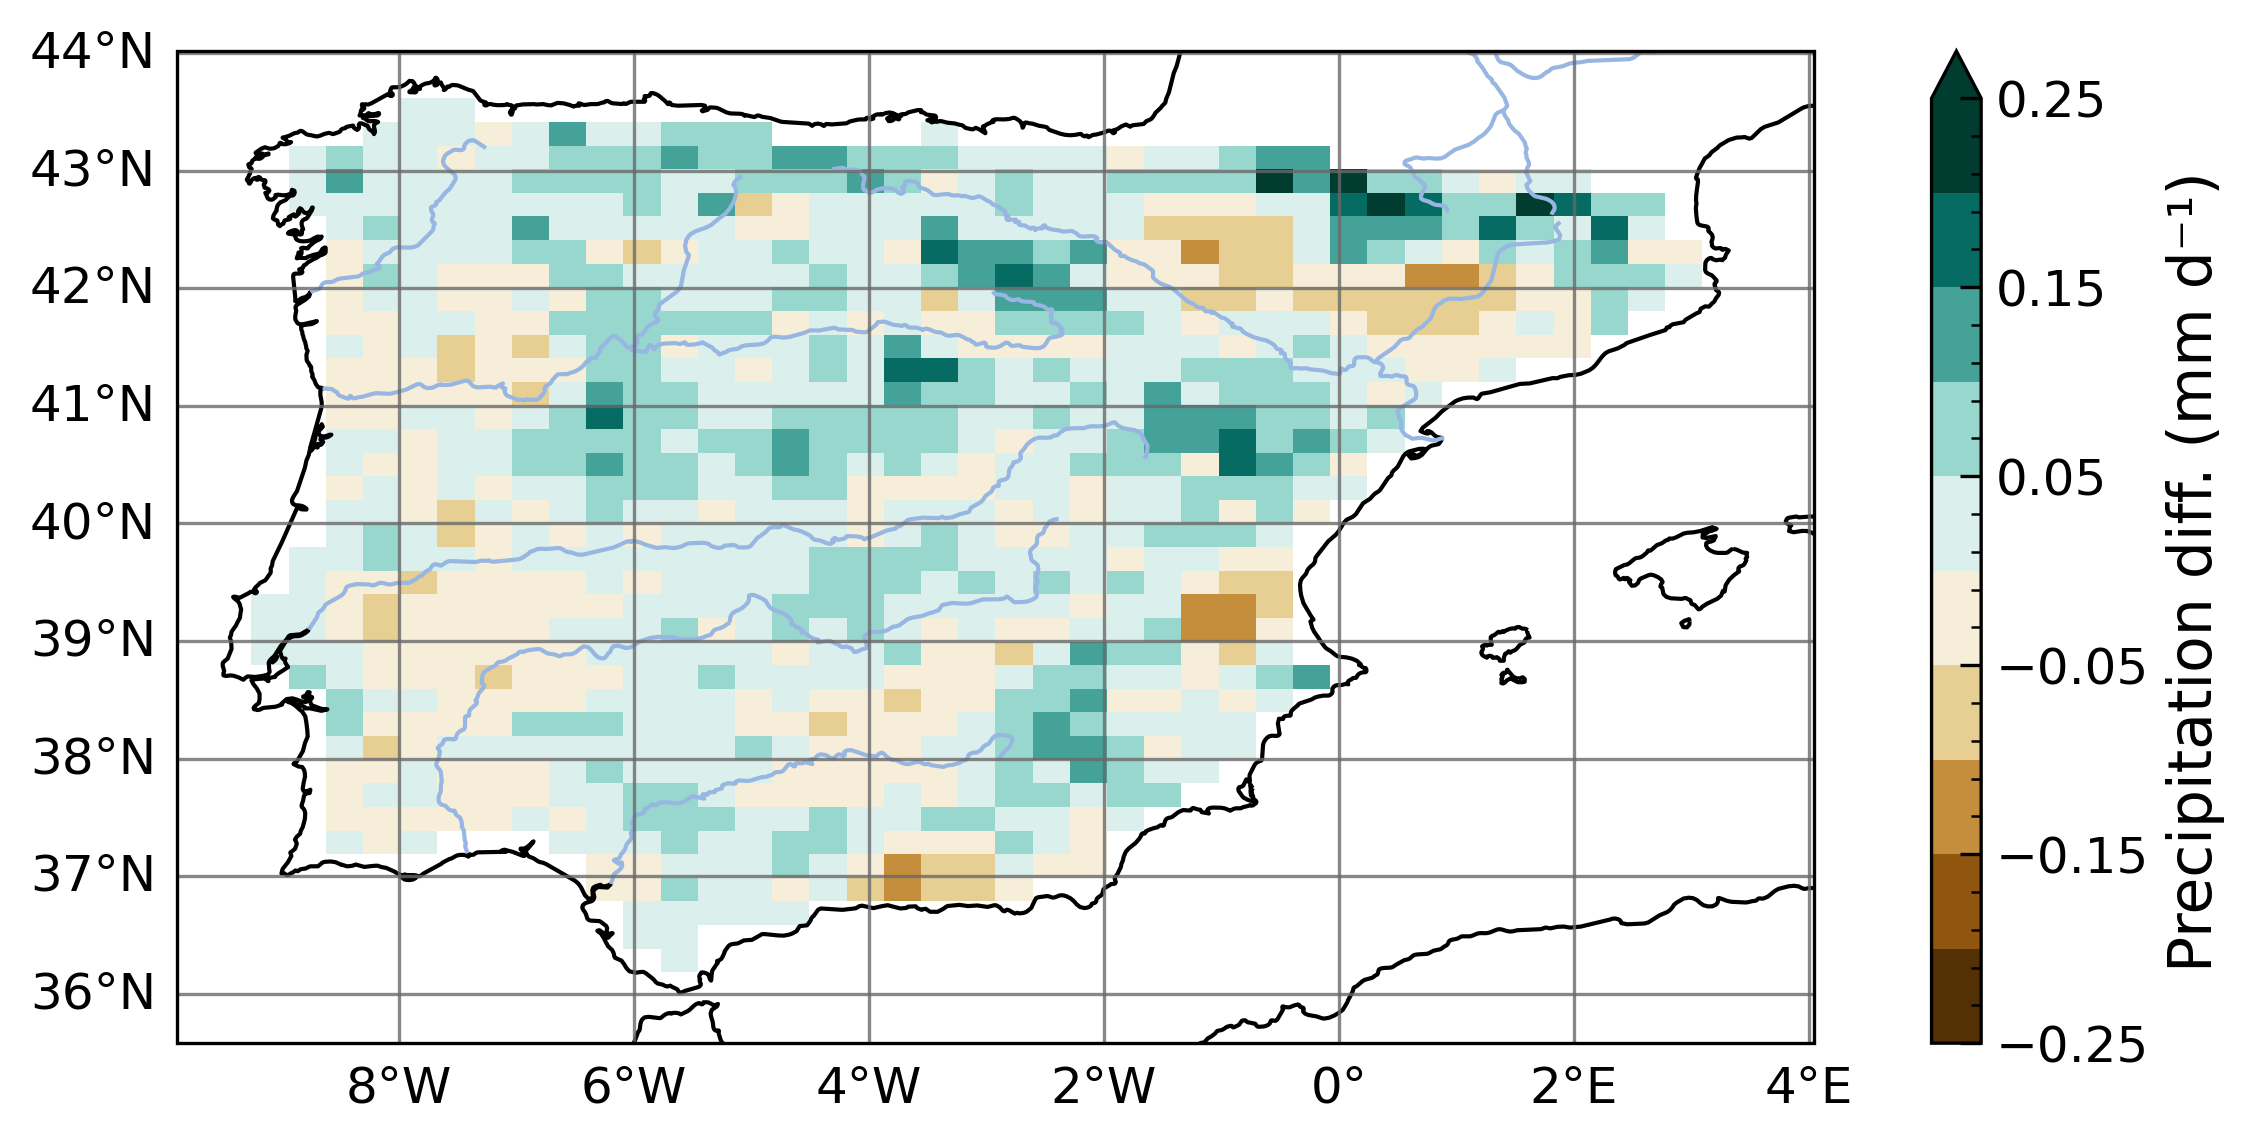
\includegraphics[width=\textwidth]{images/chap4/future/diffmap_precip_futirr.png}
        \end{subfigure} &
        %evap
        \begin{subfigure}[b]{0.5\textwidth}
            \caption{ET difference}
            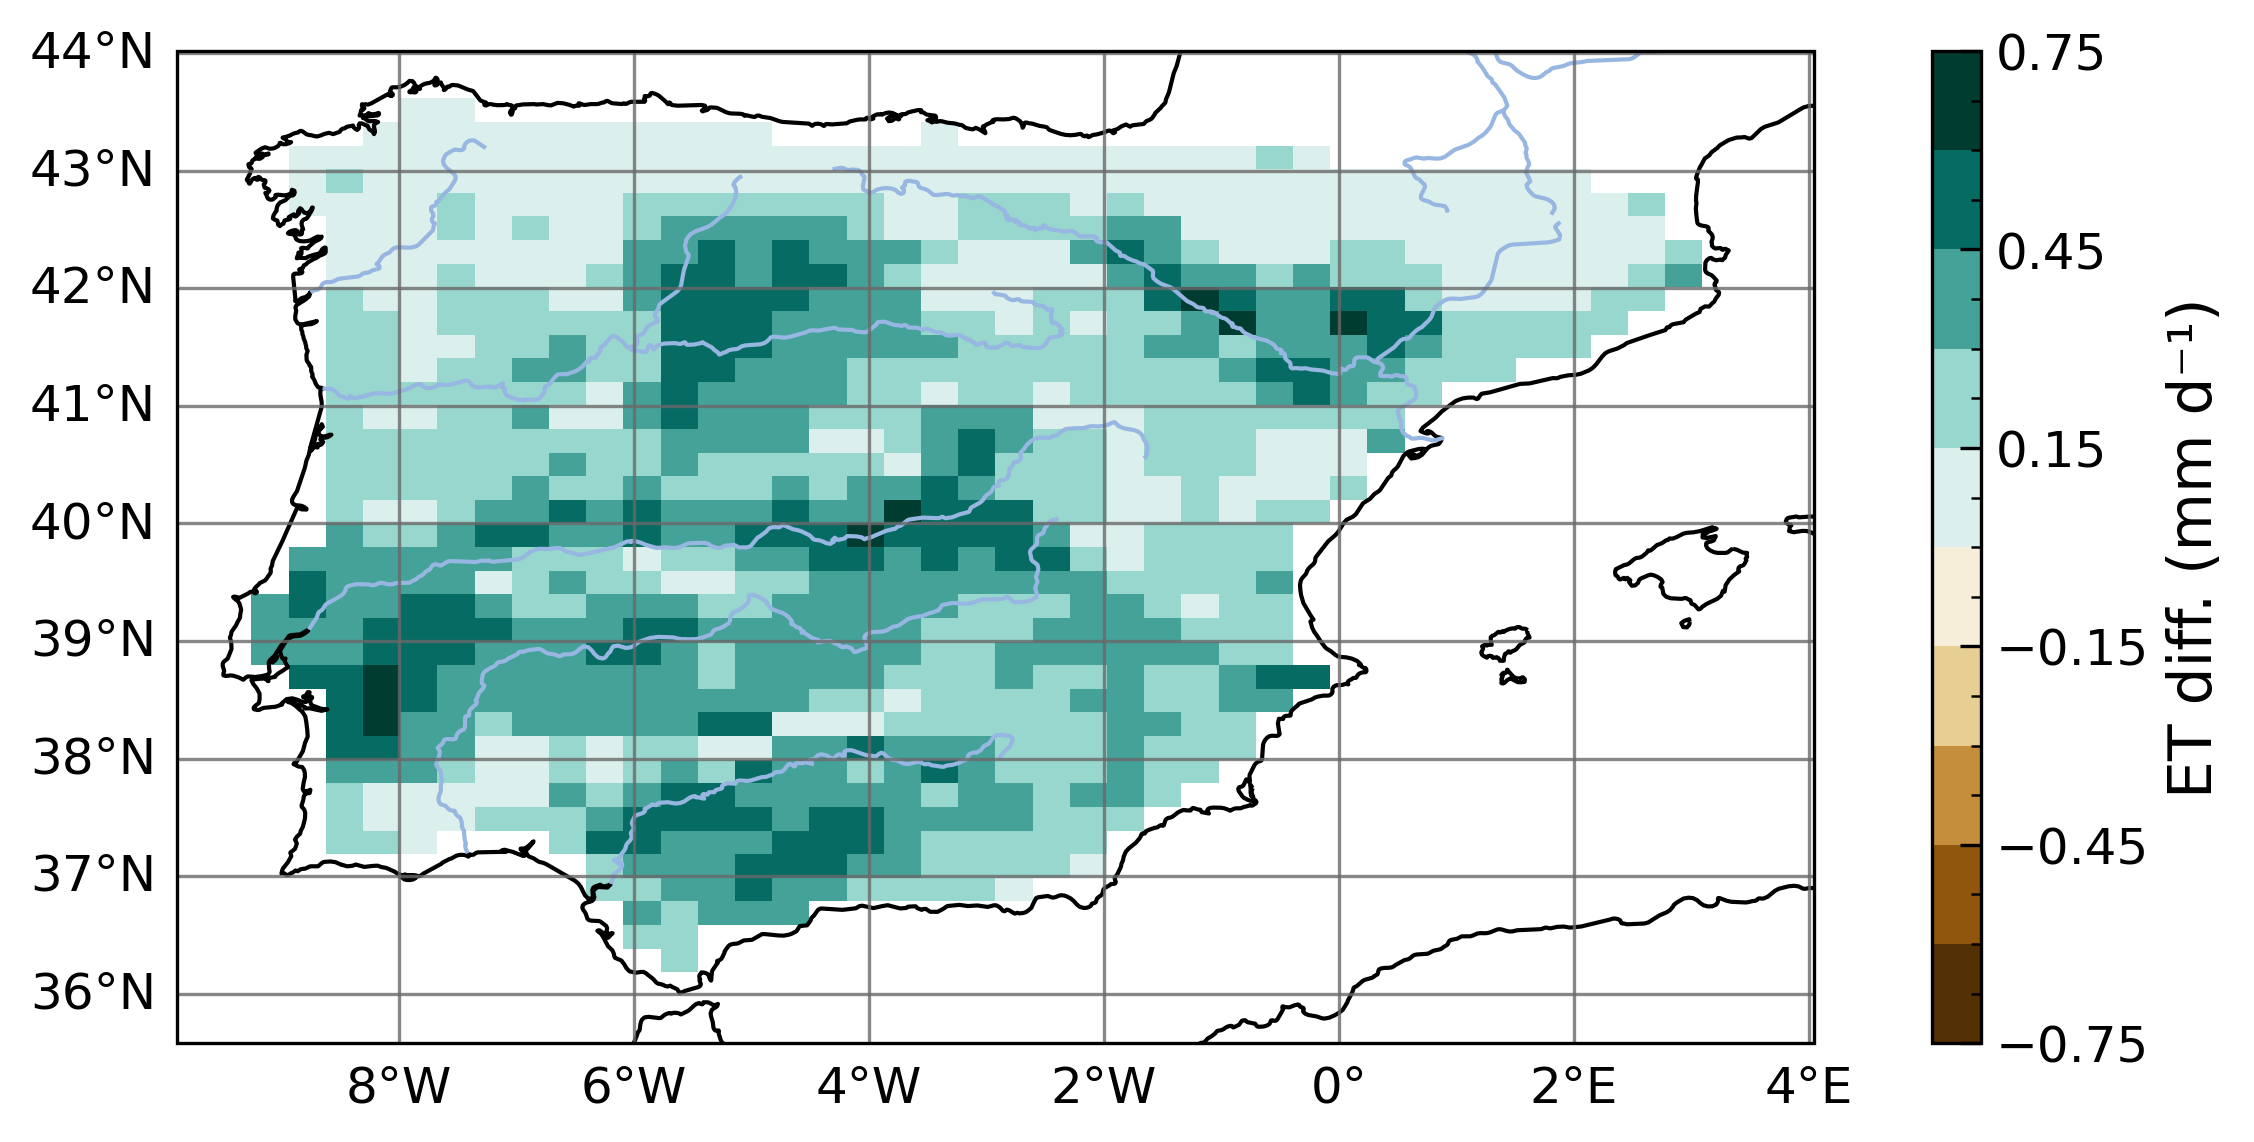
\includegraphics[width=\textwidth]{images/chap4/future/diffmap_evap_futirr.png}
        \end{subfigure} \\

        %q2m
        \begin{subfigure}[b]{0.5\textwidth}
            \caption{2-m specific humidity difference}
            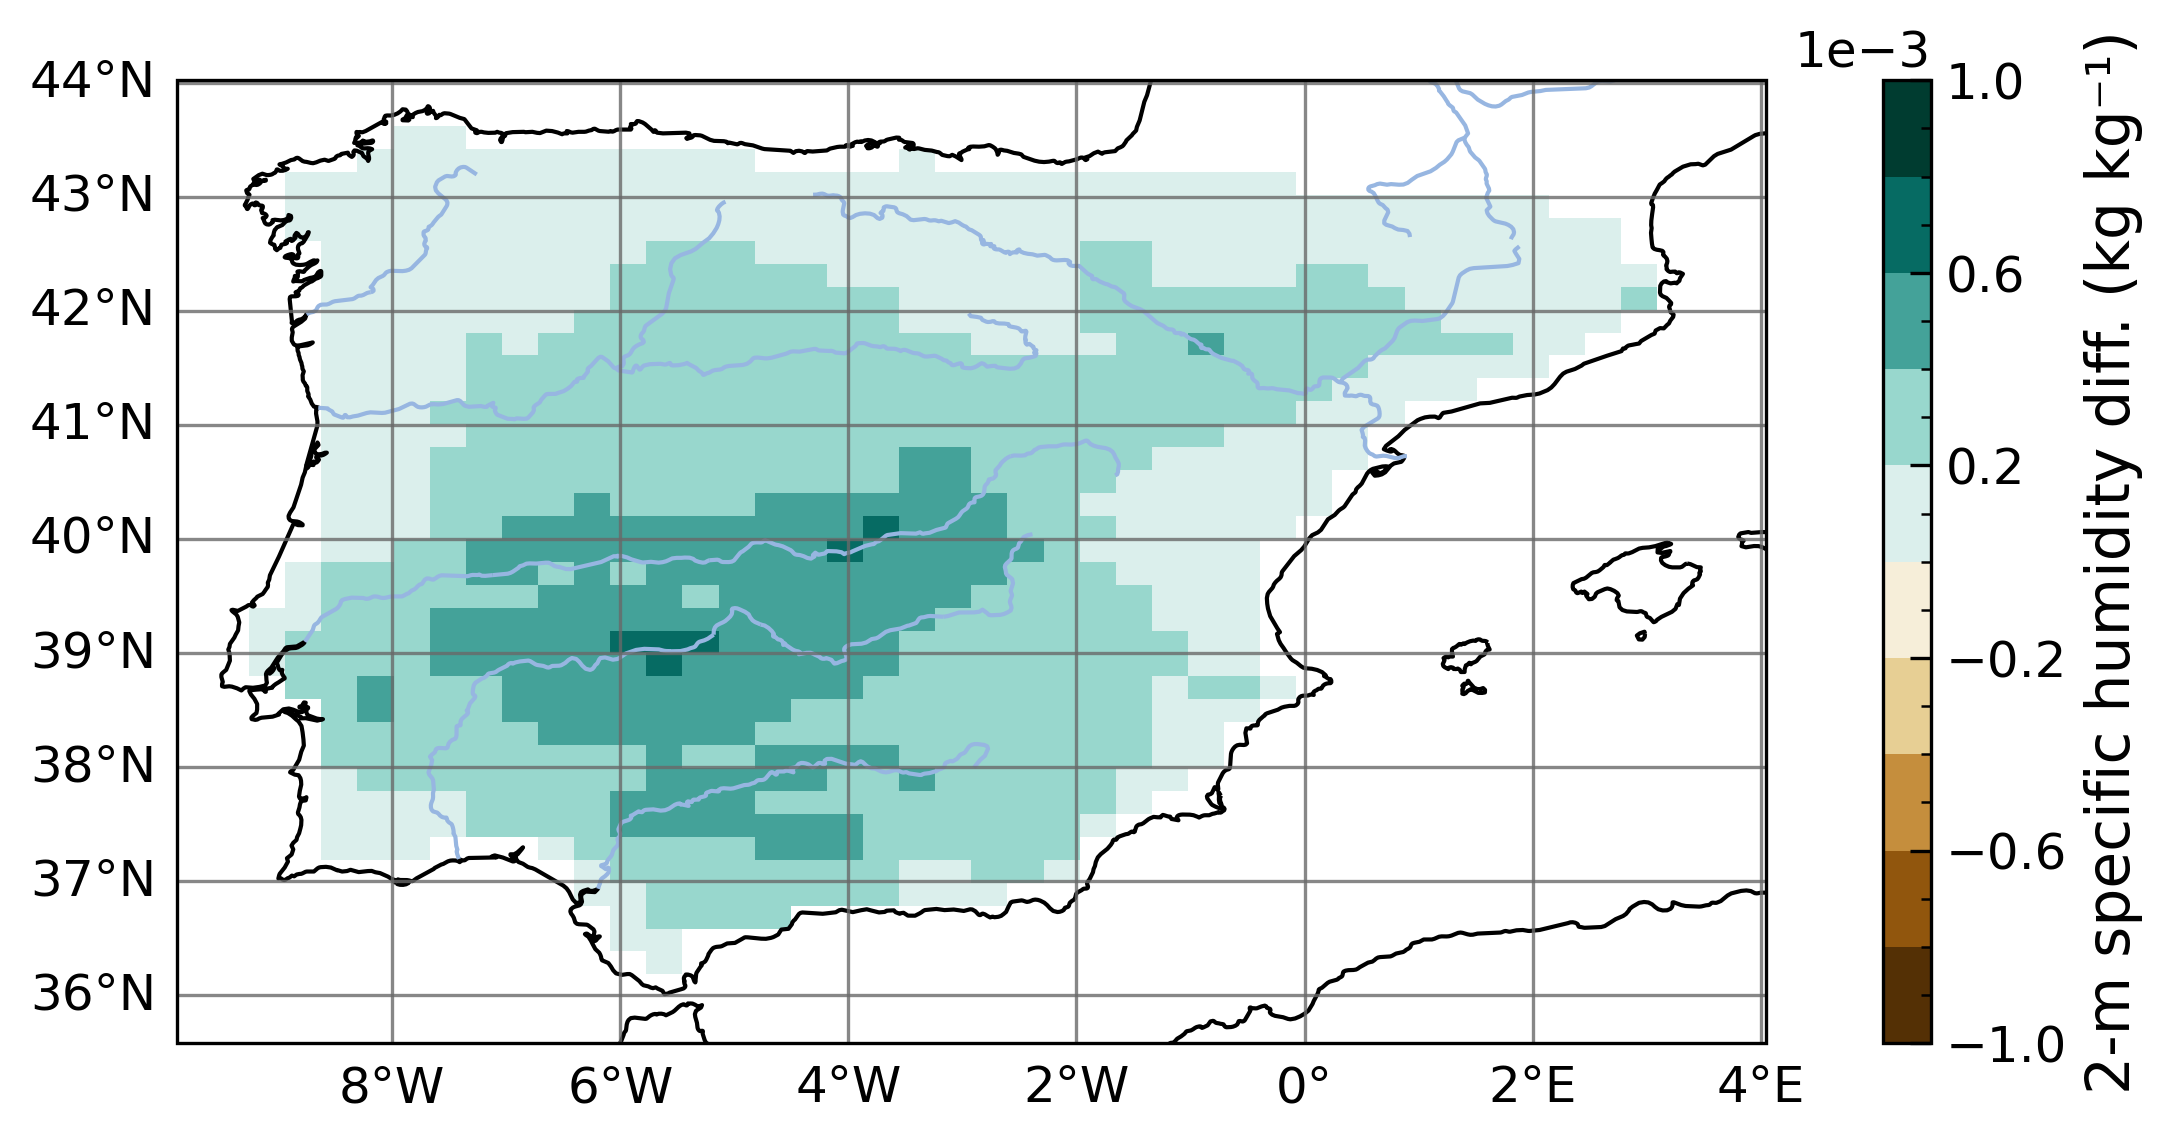
\includegraphics[width=\textwidth]{images/chap4/future/diffmap_q2m_futirr.png}
        \end{subfigure} &
        %rh2m
        \begin{subfigure}[b]{0.5\textwidth}
            \caption{2-m relative humidity difference}
            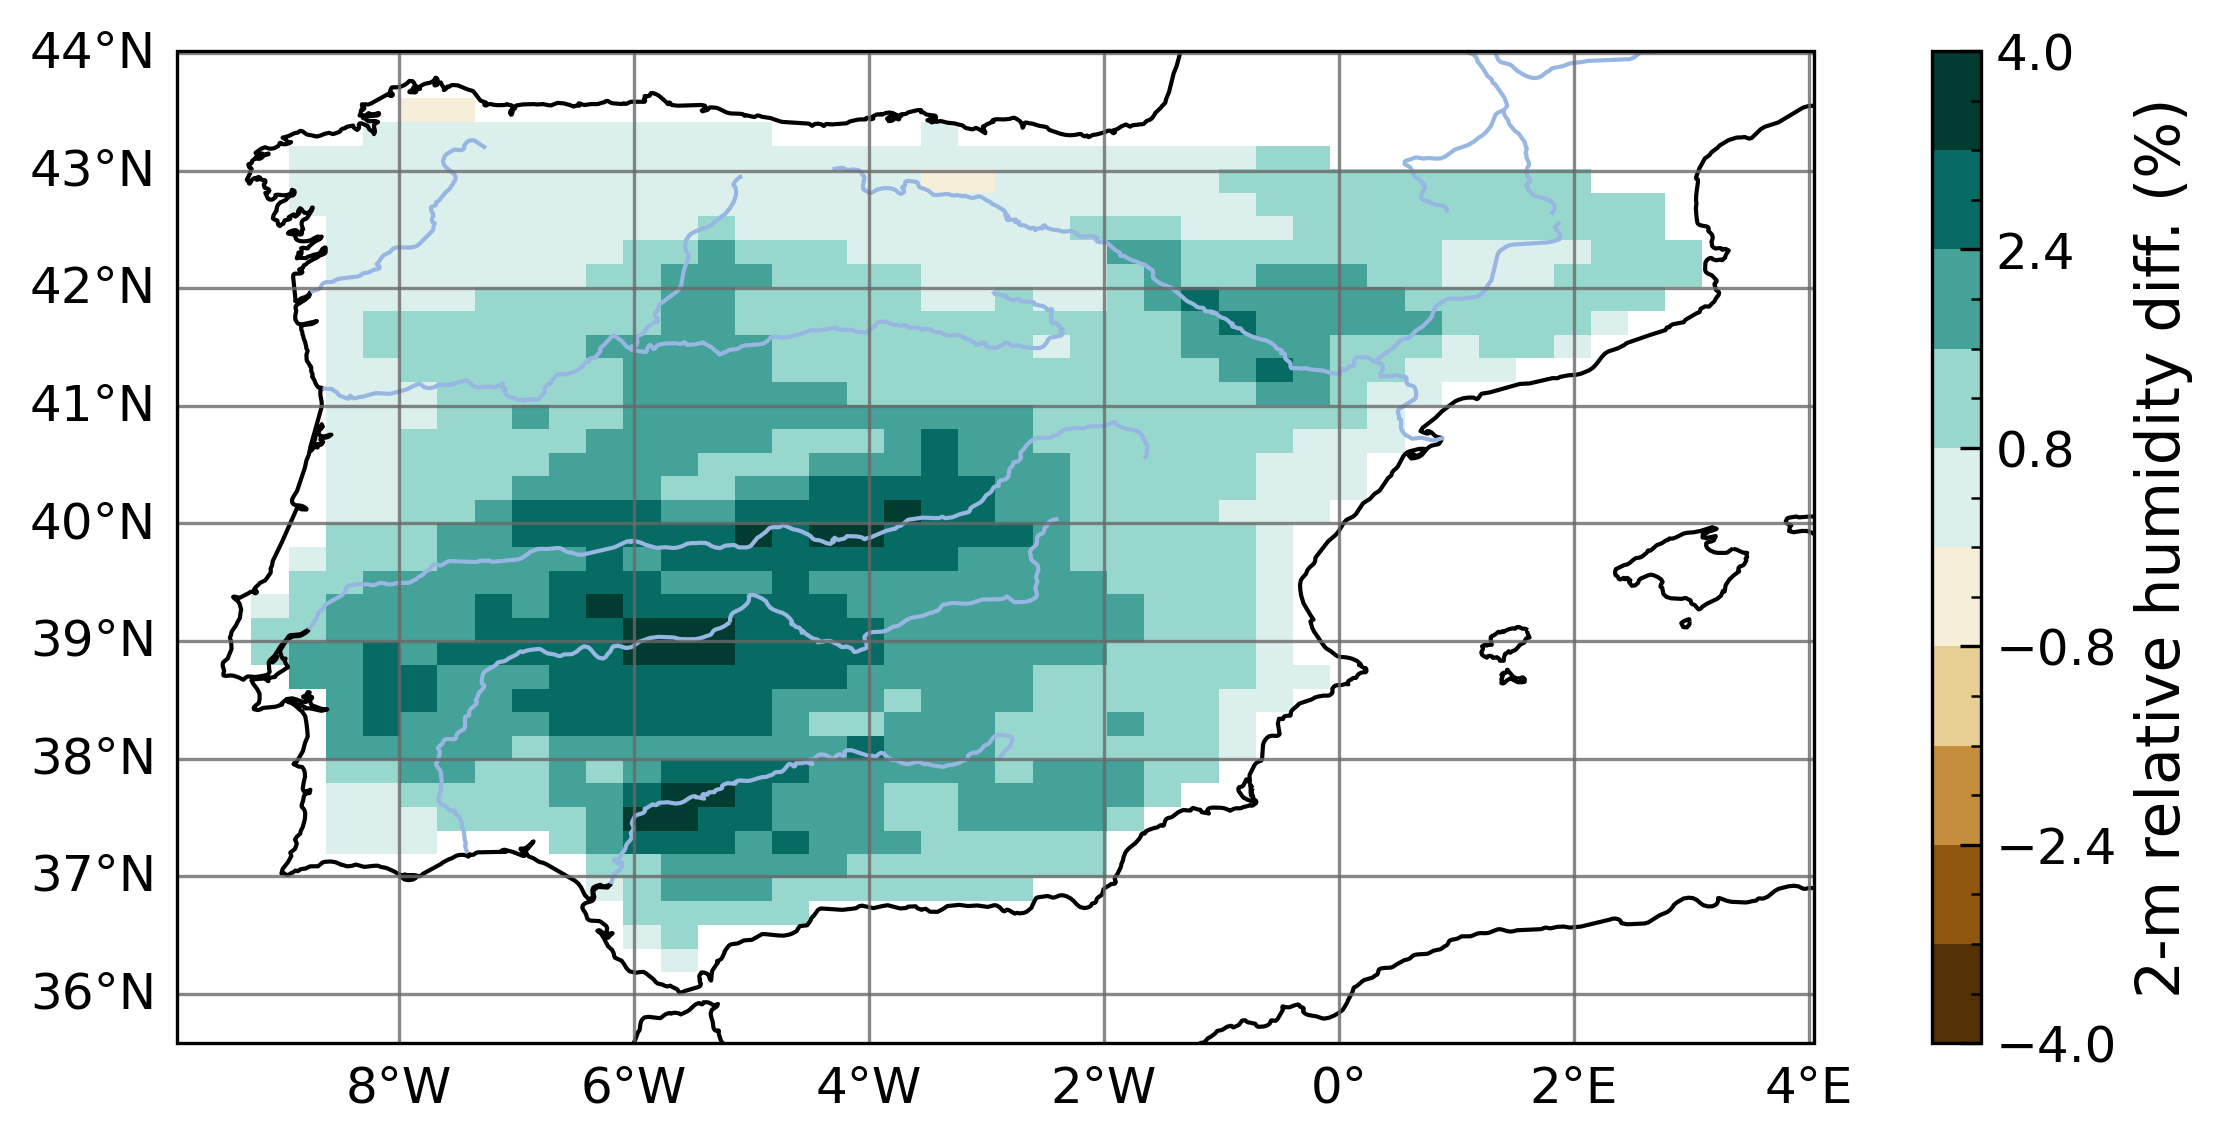
\includegraphics[width=\textwidth]{images/chap4/future/diffmap_rh2m_futirr.png}
        \end{subfigure} \\

        %pblh
        \begin{subfigure}[b]{0.5\textwidth}
            \caption{Atmospheric boundary layer height difference}
            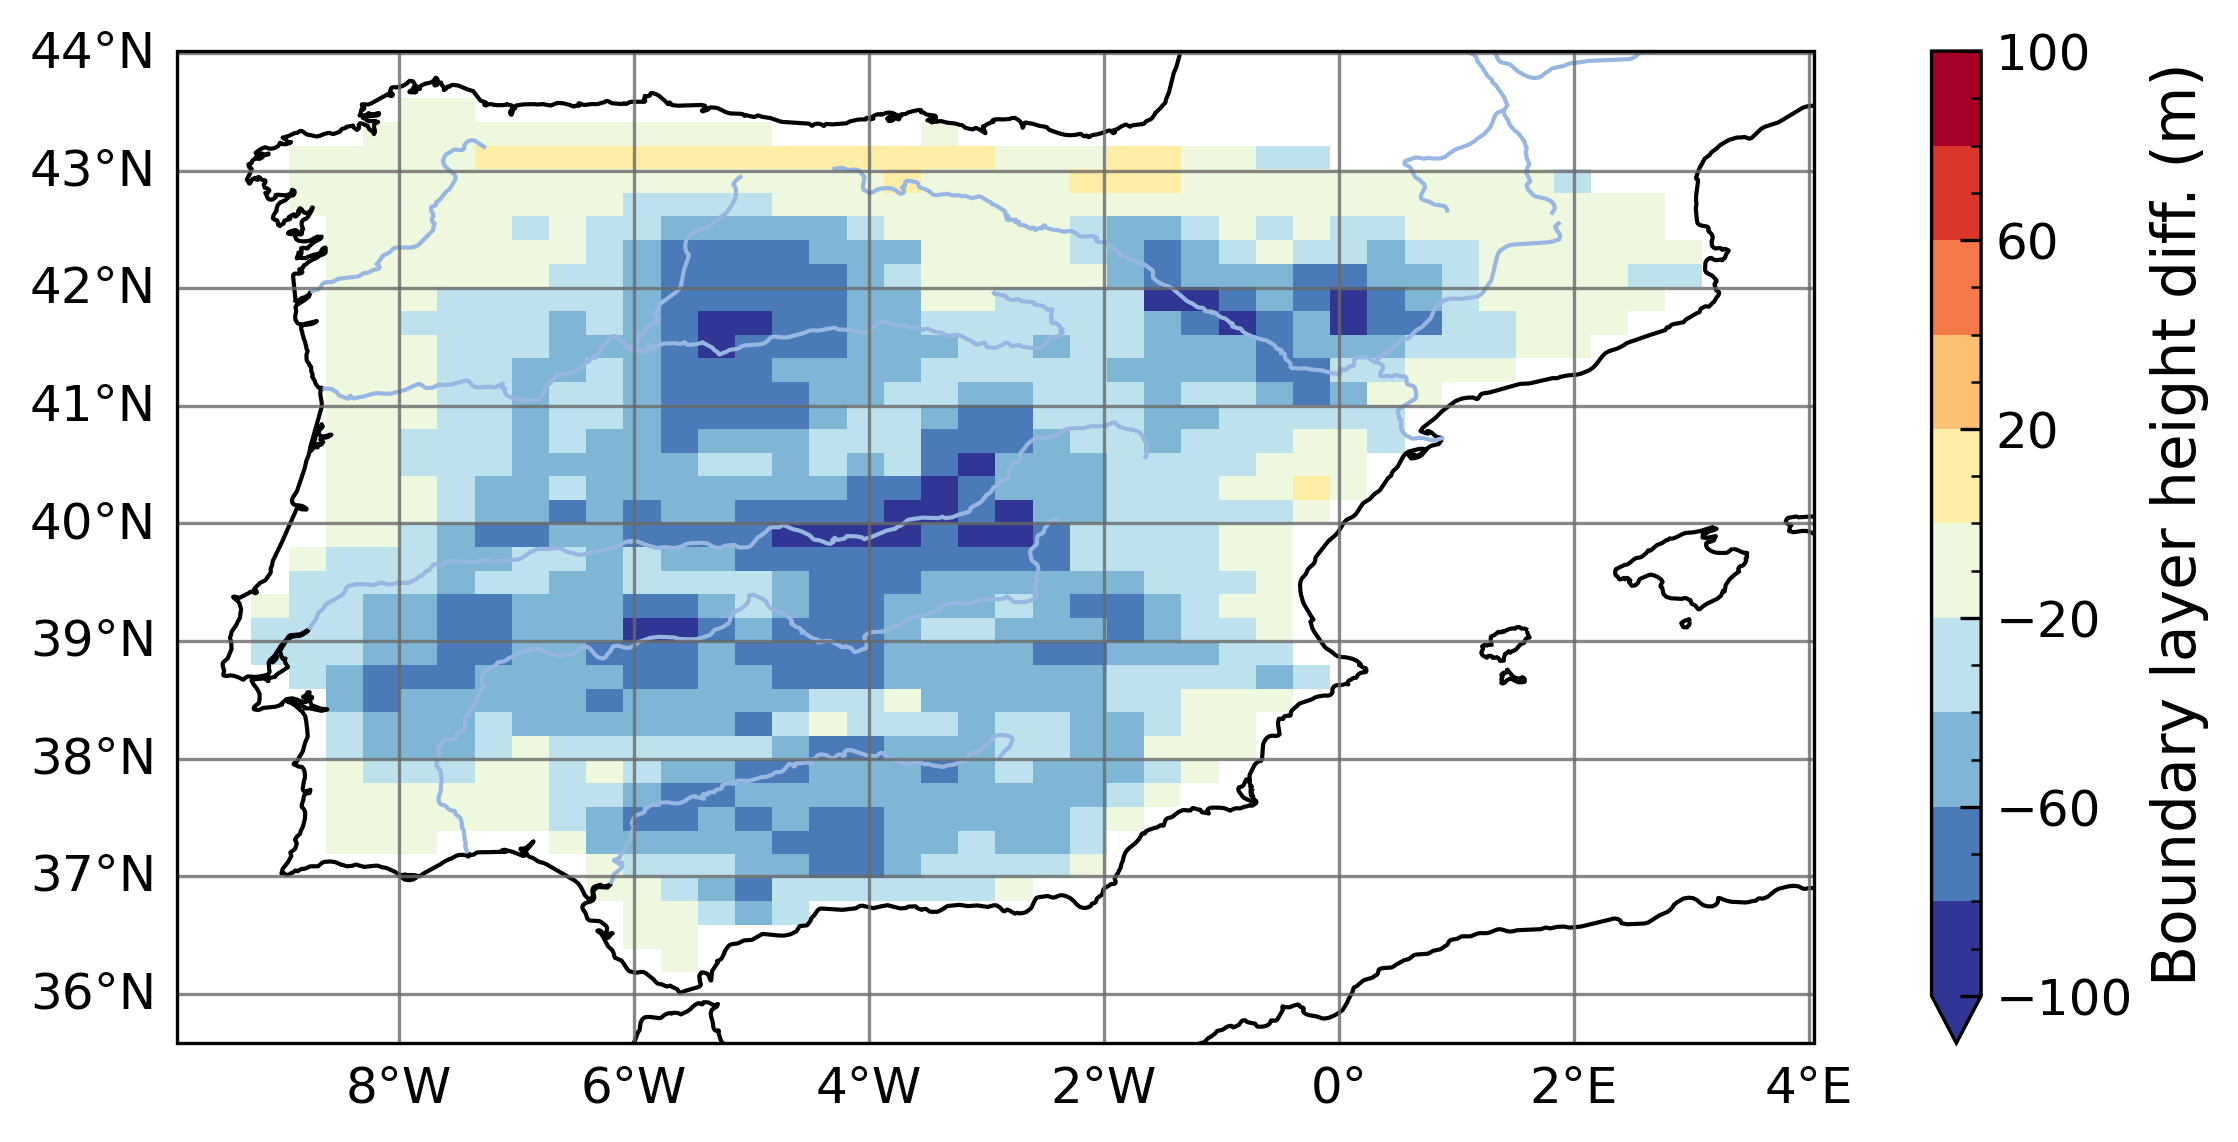
\includegraphics[width=\textwidth]{images/chap4/future/diffmap_s_pblh_futirr.png}
        \end{subfigure} &
        %lcl
        \begin{subfigure}[b]{0.5\textwidth}
            \caption{Lifting condensation level difference}
            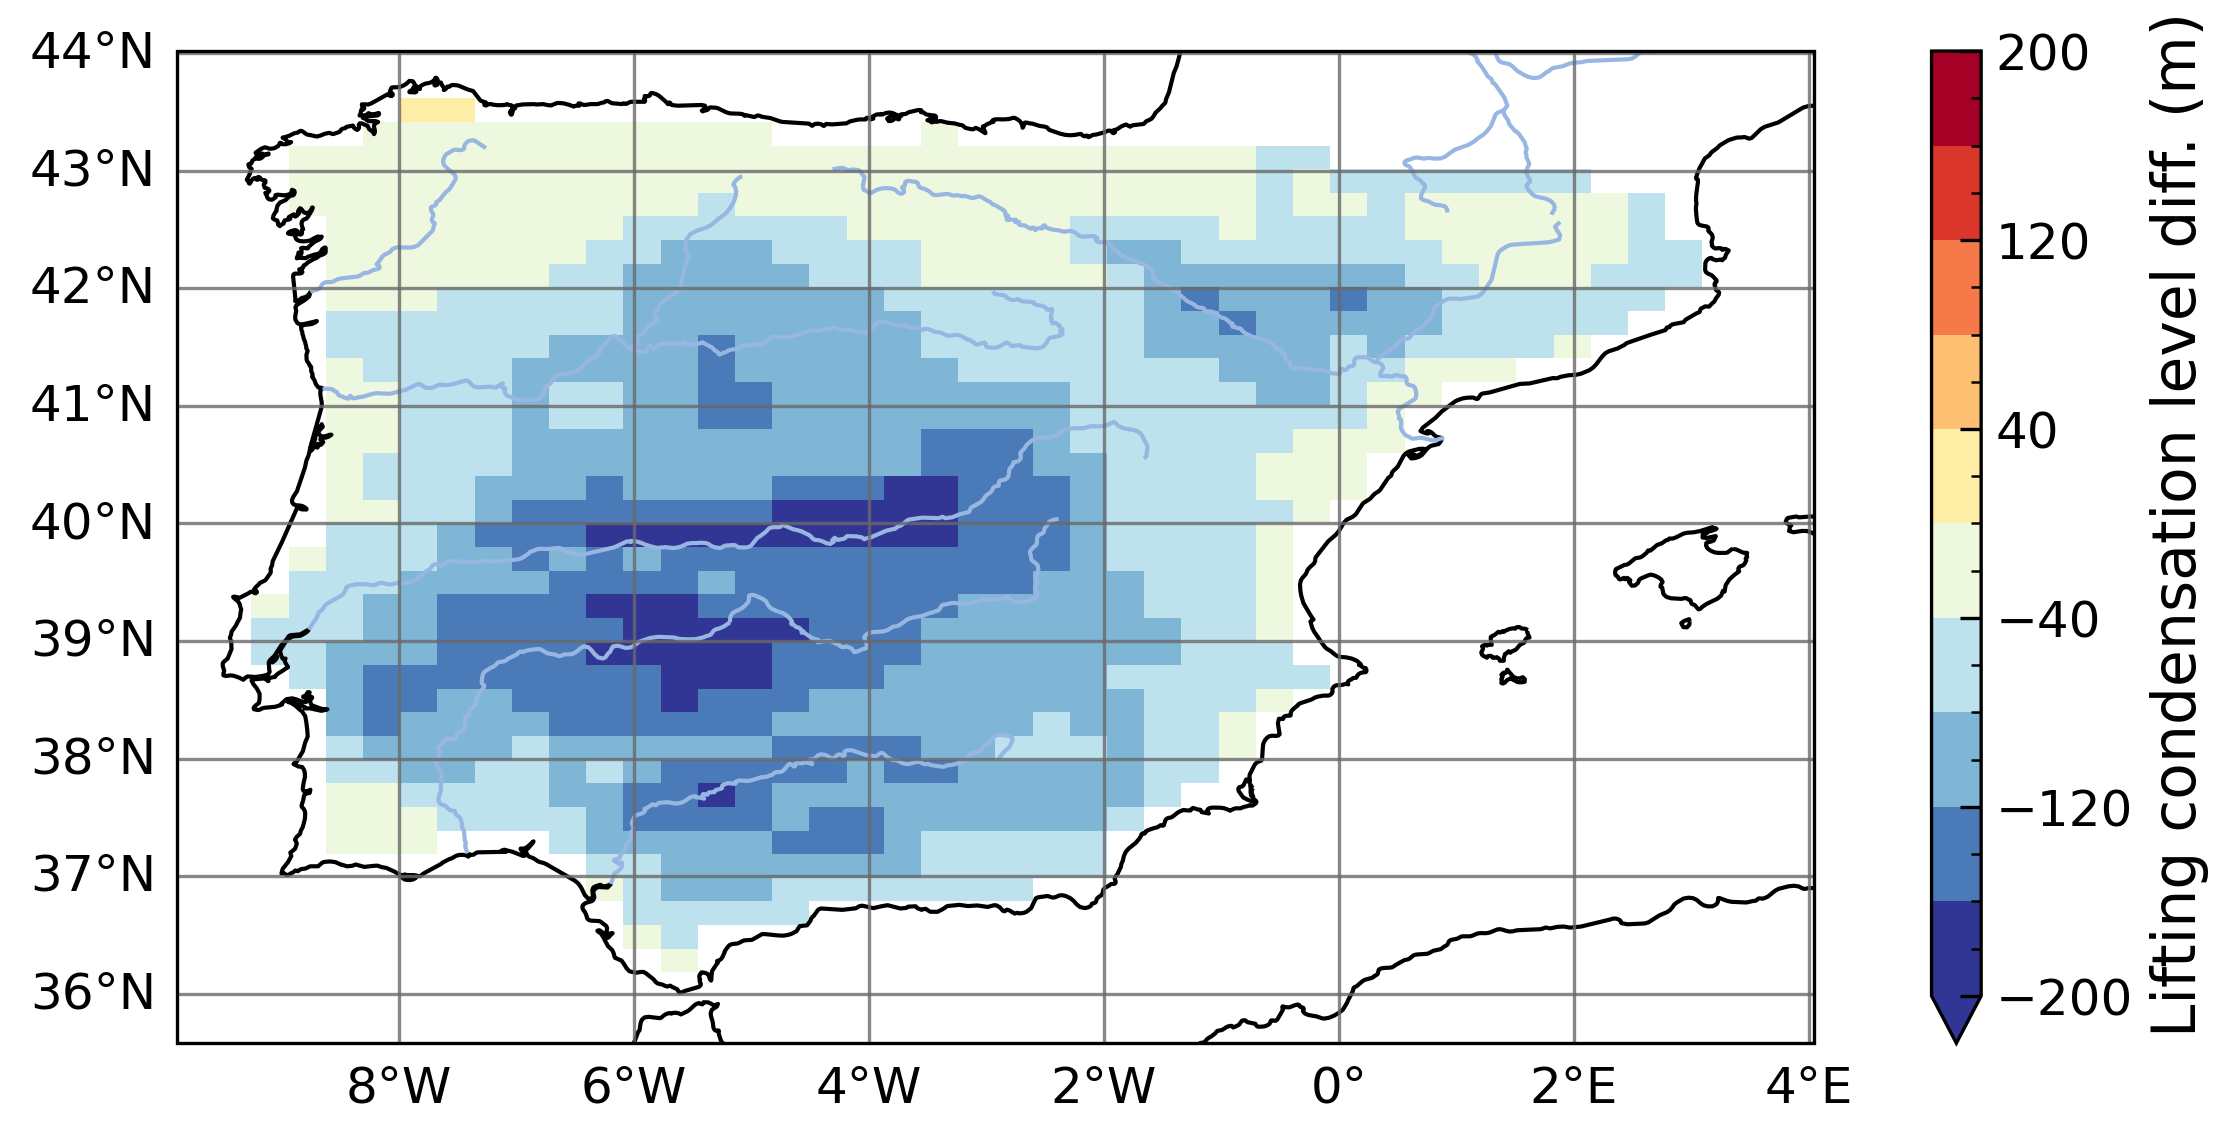
\includegraphics[width=\textwidth]{images/chap4/future/diffmap_s_lcl_futirr.png}
        \end{subfigure} \\
    \end{tabular}
    \caption{Impacts of irrigation under climate change (2050-2062). Annual mean difference between \futirr and \futnoirr.}
    \label{fig:diffmaps_future_irr}
\end{figure}

% present, no_irr : 2.18771 (mm d⁻¹)
% future, no_irr : 1.86688 (mm d⁻¹)
% future, irr : 1.89212 (mm d⁻¹)
% present, no_irr : 1.27330 (mm d⁻¹)
% future, no_irr : 1.17734 (mm d⁻¹)
% future, irr : 1.44247 (mm d⁻¹)
% present, no_irr : 14.66318 (°C)
% future, no_irr : 16.98357 (°C)
% future, irr : 16.80824 (°C)
% present, no_irr : 50.54140 (W m⁻²)
% future, no_irr : 55.53161 (W m⁻²)
% future, irr : 49.91047 (W m⁻²)
% present, no_irr : 0.00730 (kg kg⁻¹)
% future, no_irr : 0.00786 (kg kg⁻¹)
% future, irr : 0.00813 (kg kg⁻¹)
% present, no_irr : 942.46790 (m)
% future, no_irr : 946.90222 (m)
% future, irr : 909.96997 (m)
% present, no_irr : 884.01685 (m)
% future, no_irr : 1039.27222 (m)
% future, irr : 959.86011 (m)
% present, no_irr : 68.83486 (%)
% future, no_irr : 65.23708 (%)
% future, irr : 66.66062 (%)

\clearpage

\subsection{Aridification and impact of irrigation}

Aridity indices are often used as a way to characterize continental regions and how their climate will evolve in the future, under climate change. Aridity aims to describe long-term moisture deficits that limit the development of vegetation. Several definitions and indices have been proposed and used in the last decades, but the most common is the United Nations Environmental Programme (UNEP) aridity index, defined as the ratio of the annual precipitation to potential evapotranspiration : $AI = \frac{P}{PET}$. %todo:refs (Begueria 2025, UNEP 1992)
This index is most relevant when averaged over multiple years to reduce sensitivity to specific droughts or extreme precipitation events.

At the end of Mariame Maiga's internship, a short study of the evolution of aridity in ICOLMDZOR was conducted, using this index to classify grid cells into five aridity classes as presented in Table \ref{table:aridity_classes}. 
Potential evapotranspiration was taken from ORCHIDEE's \textit{evapot\_corr} variable, named $E_{pot}^*$ in the equations of Chapter \ref{chap:methods}, which is computed using the formulation of \citet{Budyko_1956} with a correction from \citet{milly_potential_1992}. 
Even though the choice of the method used to compute PET has a strong impact on the value of the aridity index and on the classification of each grid cell, this index remains an interesting tool to study the future evolution of aridity in the various regions of the Peninsula.

\begin{table}[h]
    \centering
    \begin{tabular}{|l|l|}
        \hline
        \textbf{Aridity class} & \textbf{Index values} \\
        \hline
        Hyper-arid & \( AI < 0.05 \) \\
        \hline
        Arid & \( 0.05 < AI < 0.2 \) \\
        \hline
        Semi-arid & \( 0.2 < AI < 0.5 \) \\
        \hline
        Dry sub-humid & \( 0.5 < AI < 0.65 \) \\
        \hline
        Humid & \( 0.65 < AI \) \\
        \hline
    \end{tabular}
    \caption{Aridity classes based on UNEP aridity index values.}
    \label{table:aridity_classes}
\end{table}

The spatial distribution in the \presnoirr simulation (Fig. \ref{fig:aridity_index_v2}a, b) shows a dominant semi-arid climate over the Iberian Peninsula, with a humid strip in the northern coast and the Pyrenees, and arid climate in the Ebro and Guadalquivir valleys, and other areas in the South.
Under the SSP5-8.5 climate change scenario, in \futnoirr (Fig. \ref{fig:aridity_index_v2}c, d), the share of humid grid cells falls from 16.5\% to 6.8\%, and the share of semi-arid from 58.6\% to 50.1\%, while the share or arid grid cells doubles, from 18.5\% to 36.1\%. This corresponds to a shift in each aridity class. Most humid areas change to dry sub-humid or even directly to semi-arid, leaving only the heart of the Pyrenees and of the Cantabrian mountain ranges in this aridity class. The arid areas, on the contrary, extend to encompass a large share of the Ebro, Guadiana and Guadalquivir basins, and the central part of the Tagus valley. This shift in aridity is consistent with the changes described in Fig. \ref{fig:diffmaps_present_future}, a decrease of precipitation and an increase in temperature which partly drives PET. %option:show evapot_corr evolution ? 

The influence of irrigation on this evolution under climate change remains limited (Fig. \ref{fig:aridity_index_v2}). The share of arid grid cells is lower in \futirr (29.4\%) than \futnoirr (36.1\%), which is mostly compensated by a larger share of semi-arid grid cells (55.4\% instead of 50.1\%) wheareas the share of dry sub-humid and humid cells increase by lass than one percentage point.
This impact is mostly visible in the northwestern part of the Peninsula, and in the mountain ranges on both sides of the Guadalquivir valley, the Sierra Morena (which separates it from the Guadiana basin) and the Betic System (in the South East). Irrigation has an effect on the aridity index through the moistening and cooling of the lower atmosphere, which can decrease PET, and through the changes in precipitation. As described in Fig. \ref{fig:diffmaps_future_irr}, the cooling induced by irrigation is rather small compared to the warming induced by climate change, and the increases in precipitation are mostly located in the elevated areas. This explains why irrigation is not able to limit the expansion of the arid areas in the valleys under climate change, and mostly affects aridity in the mountainous regions. This result is clearly dependent on the choice of the aridity index, but in practical terms, it points to the fact that irrigation is an adaptation strategy which can help sustaining plant growth in the valleys, but with limited long-term benefits on the local climate over cultivated areas.

%figure : maps of aridity index classes for present and future
\begin{figure}[htbp]
    \centering
    %pres, no_irr
    \begin{subfigure}[b]{0.67\textwidth}
        \caption{Aridity index classes in \presnoirr (2010-2022)}
        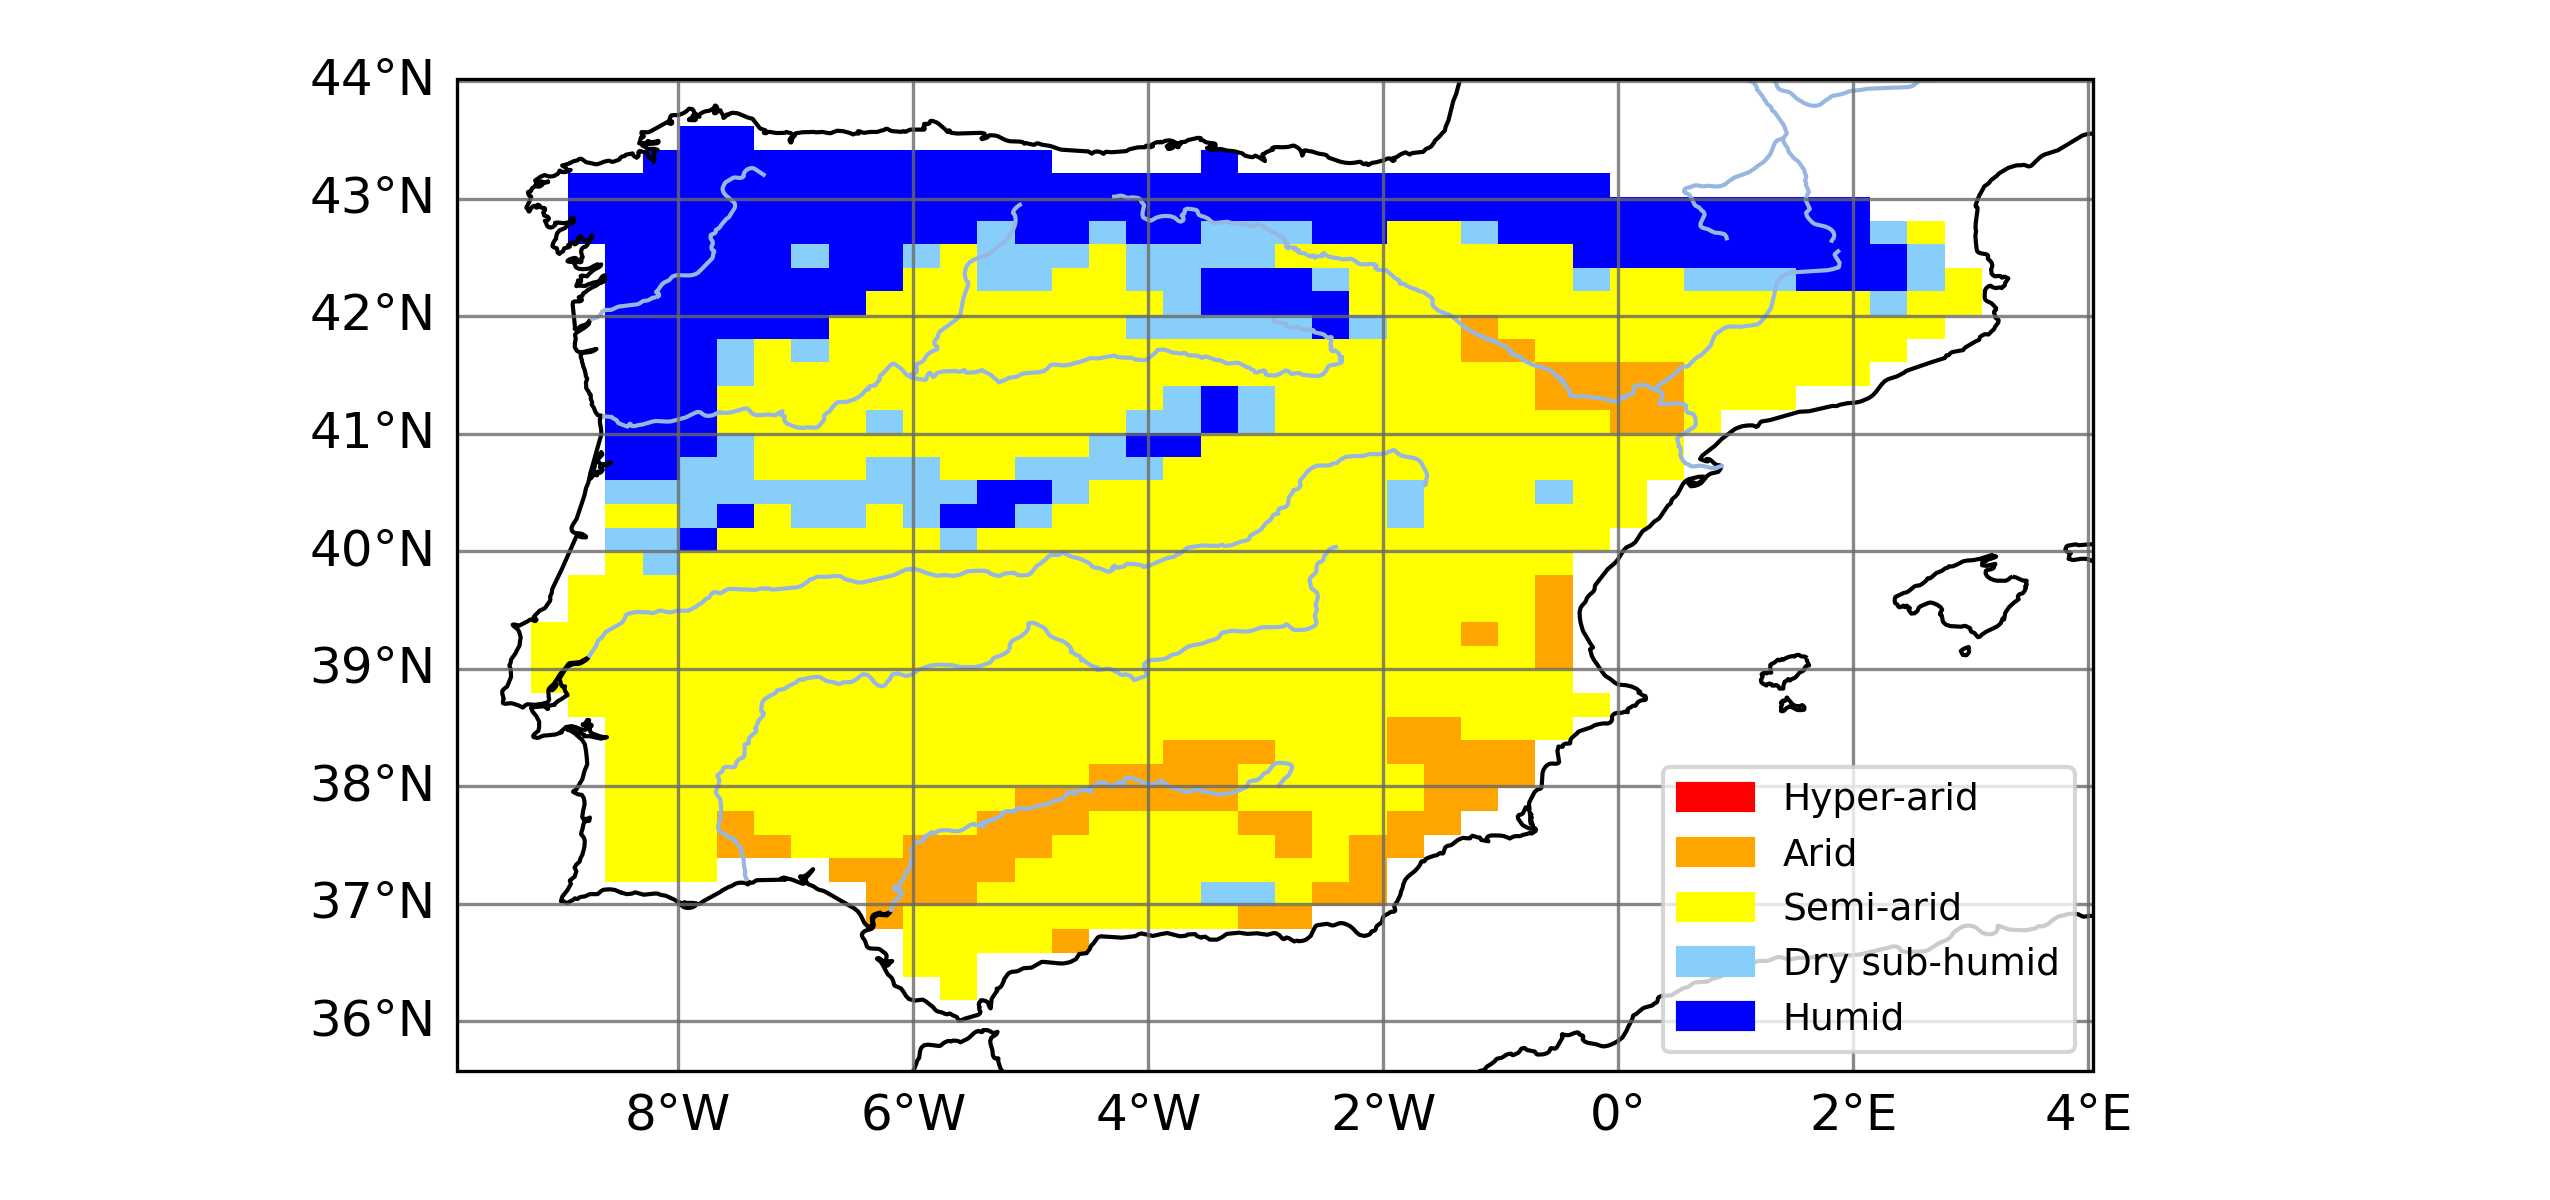
\includegraphics[width=\textwidth]{images/chap4/future/aridity_index_pres_noirr.png}
    \end{subfigure}
    \begin{subfigure}[b]{0.31\textwidth}
        \caption{Share of aridity index classes in \presnoirr (2010-2022)}
        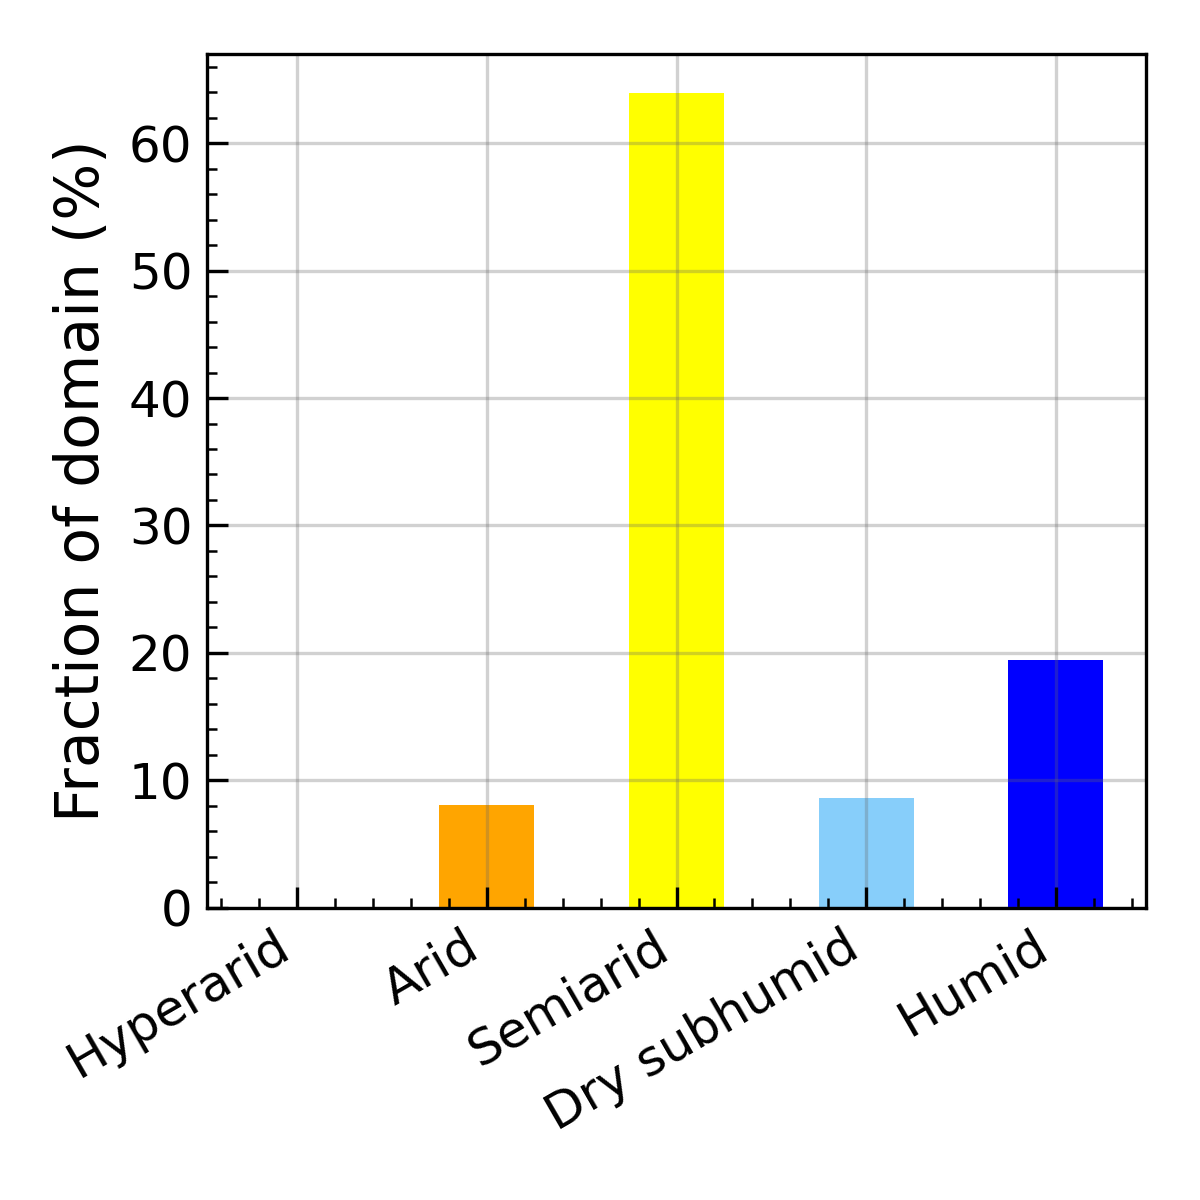
\includegraphics[width=\textwidth]{images/chap4/future/aridity_index_distribution_pres_noirr.png}
    \end{subfigure} \\

    %future, noirr
    \begin{subfigure}[b]{0.67\textwidth}
        \caption{Aridity index classes in \futnoirr (2050-2062)}
        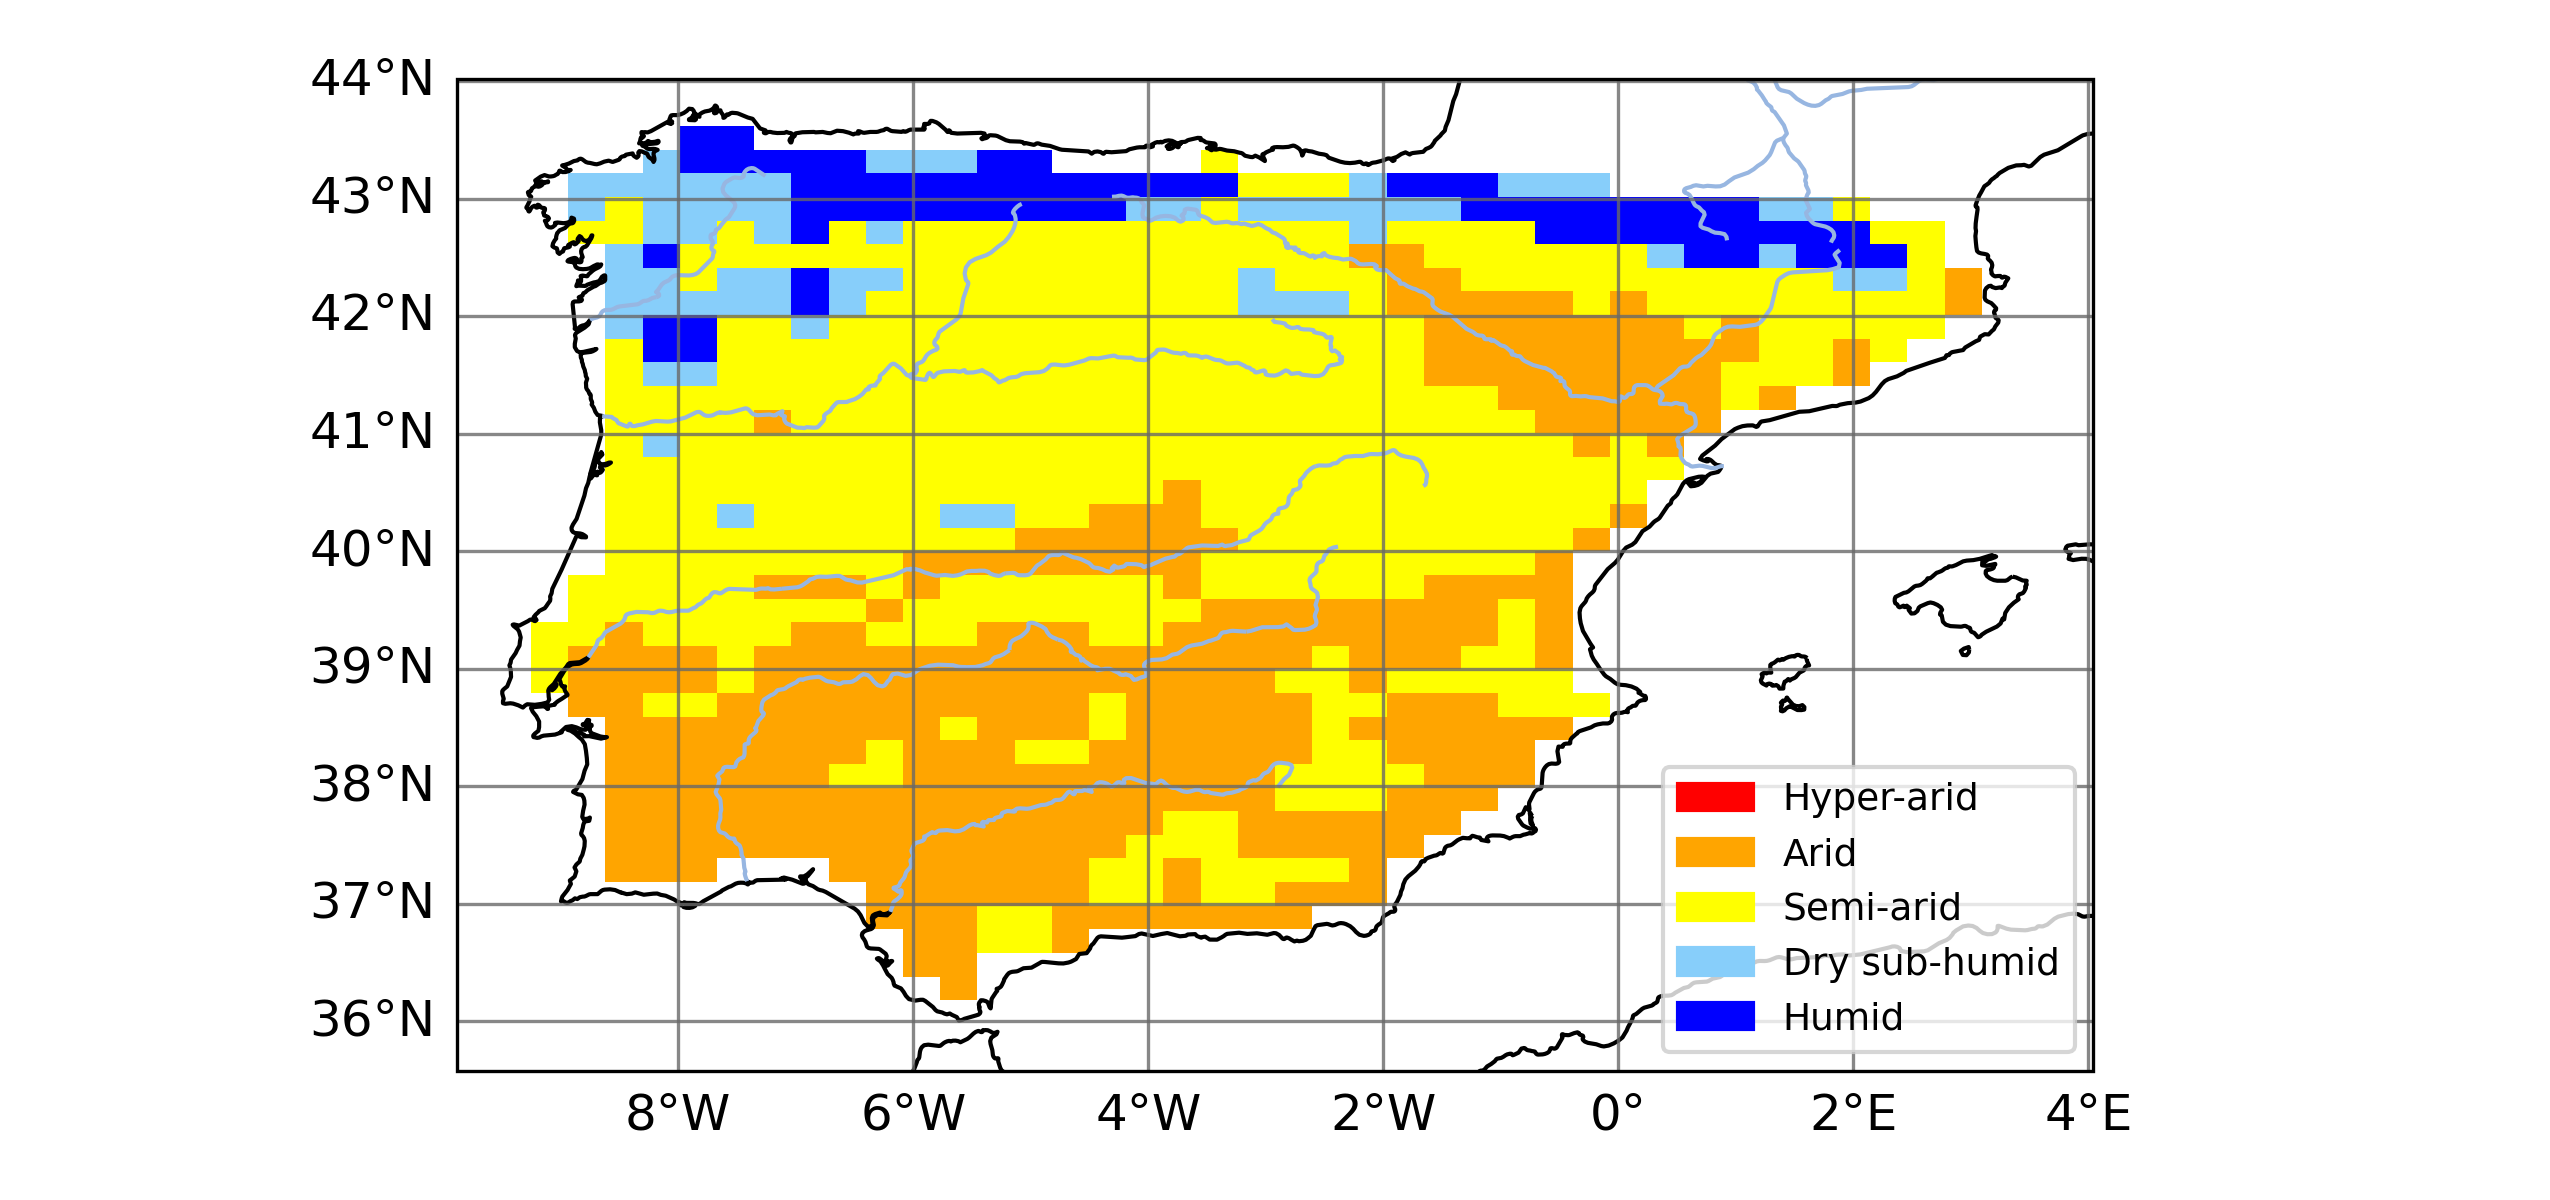
\includegraphics[width=\textwidth]{images/chap4/future/aridity_index_fut_noirr.png}
    \end{subfigure}
    \begin{subfigure}[b]{0.31\textwidth}
        \caption{Share of aridity index classes in \futnoirr (2050-2062)}
        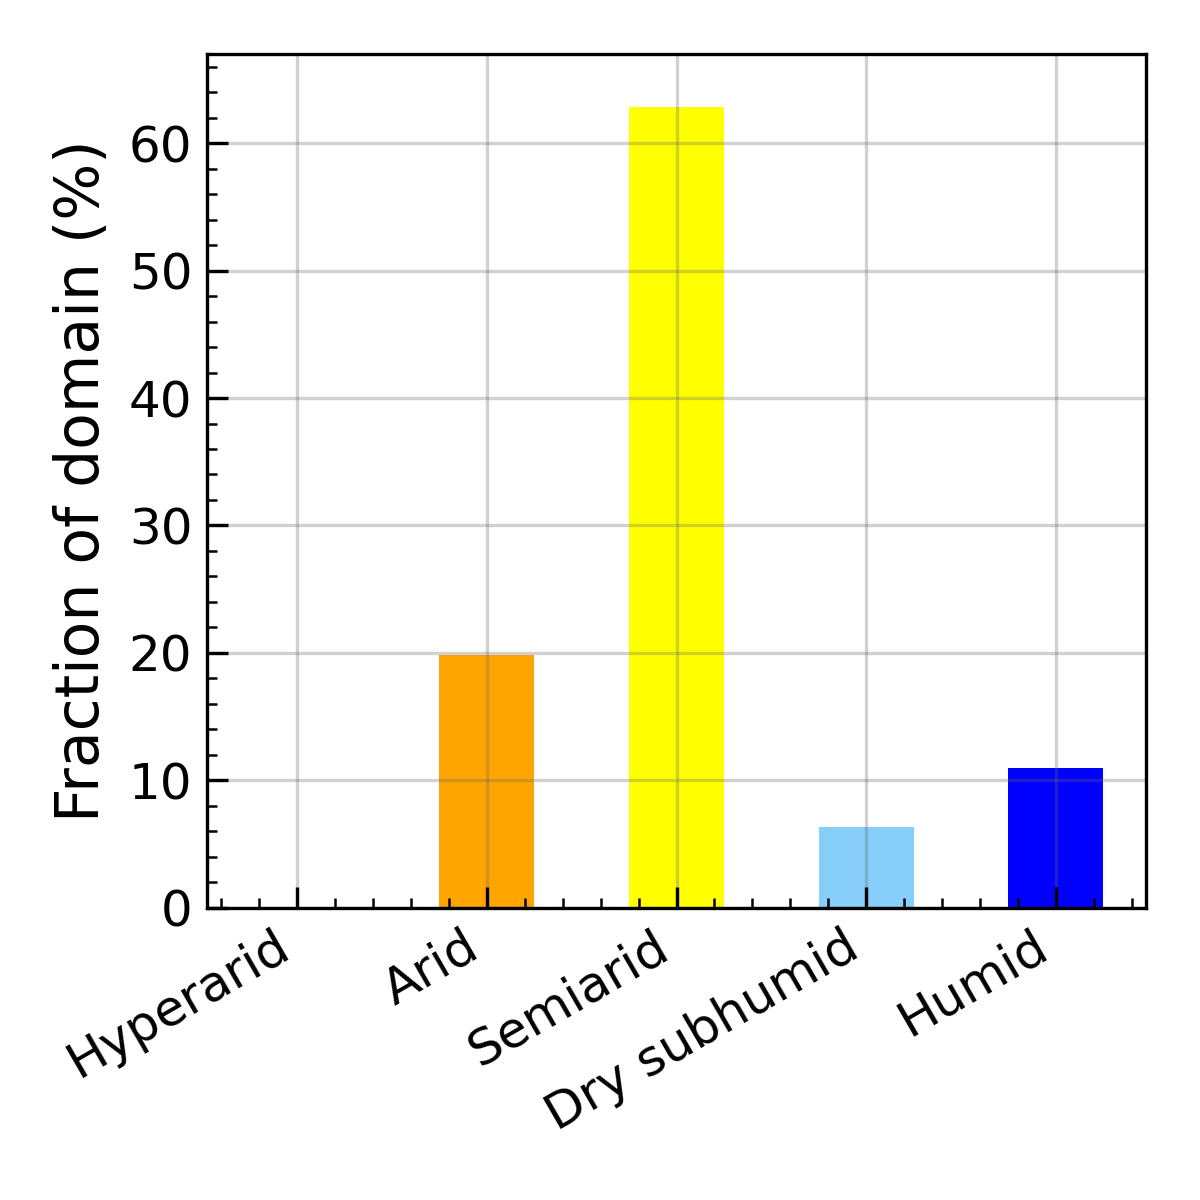
\includegraphics[width=\textwidth]{images/chap4/future/aridity_index_distribution_fut_noirr.png}
    \end{subfigure} \\

    %future, irr
    \begin{subfigure}[b]{0.67\textwidth}
        \caption{Aridity index classes in \futirr (2050-2062)}
        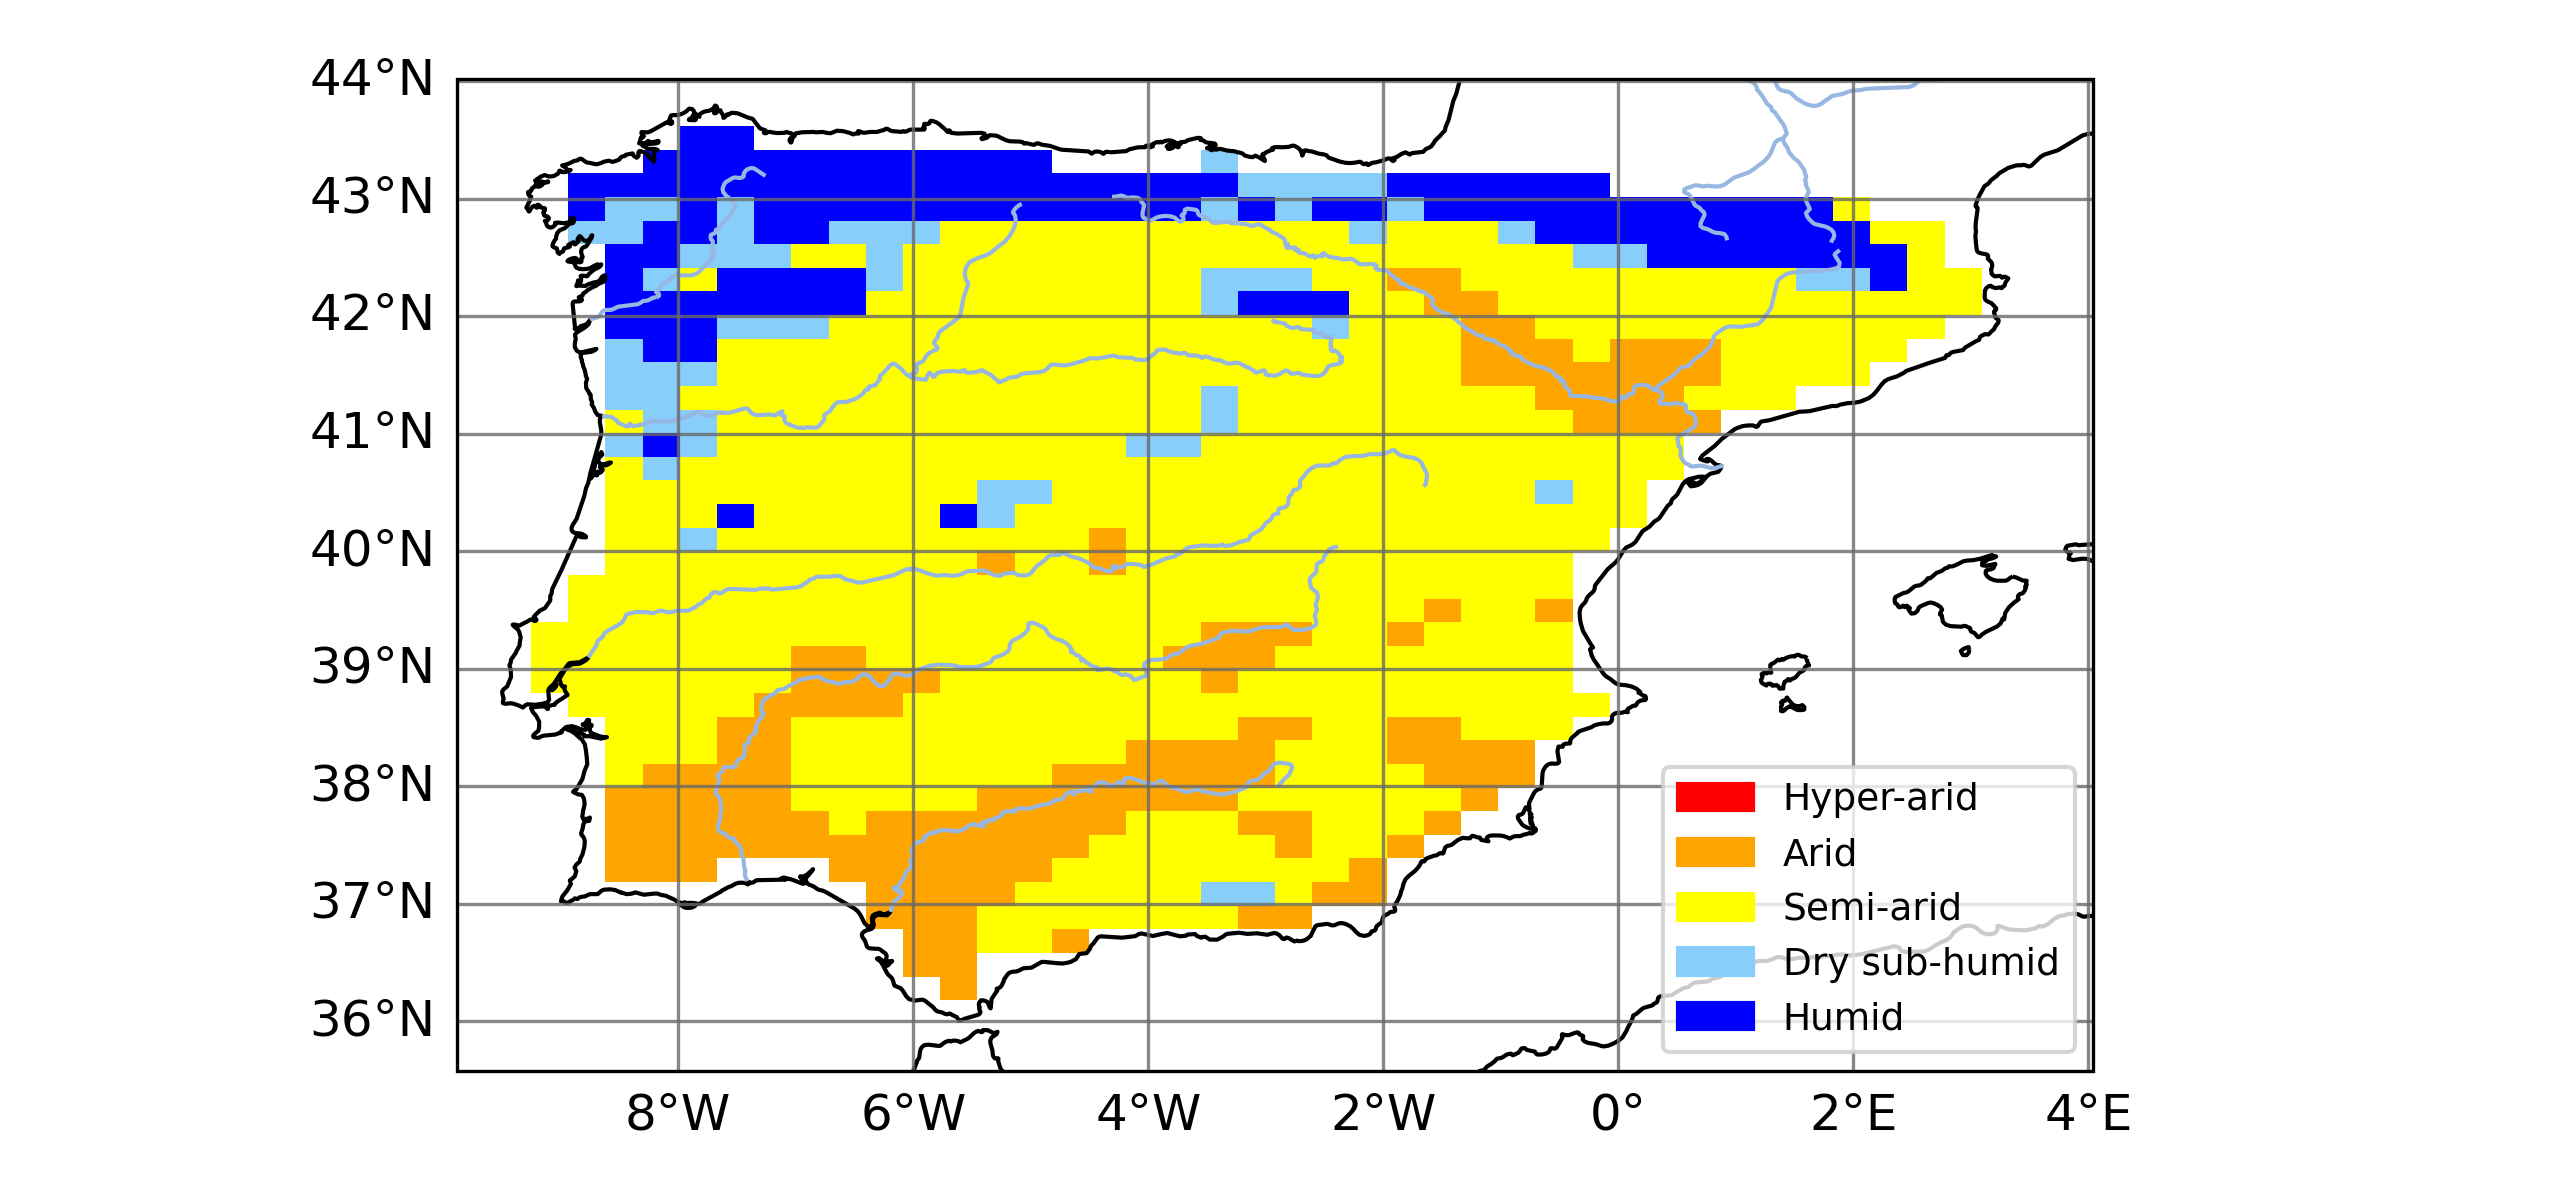
\includegraphics[width=\textwidth]{images/chap4/future/aridity_index_fut_irr.png}
    \end{subfigure}
    \begin{subfigure}[b]{0.31\textwidth}
        \caption{Share of aridity index classes in \futirr (2050-2062)}
        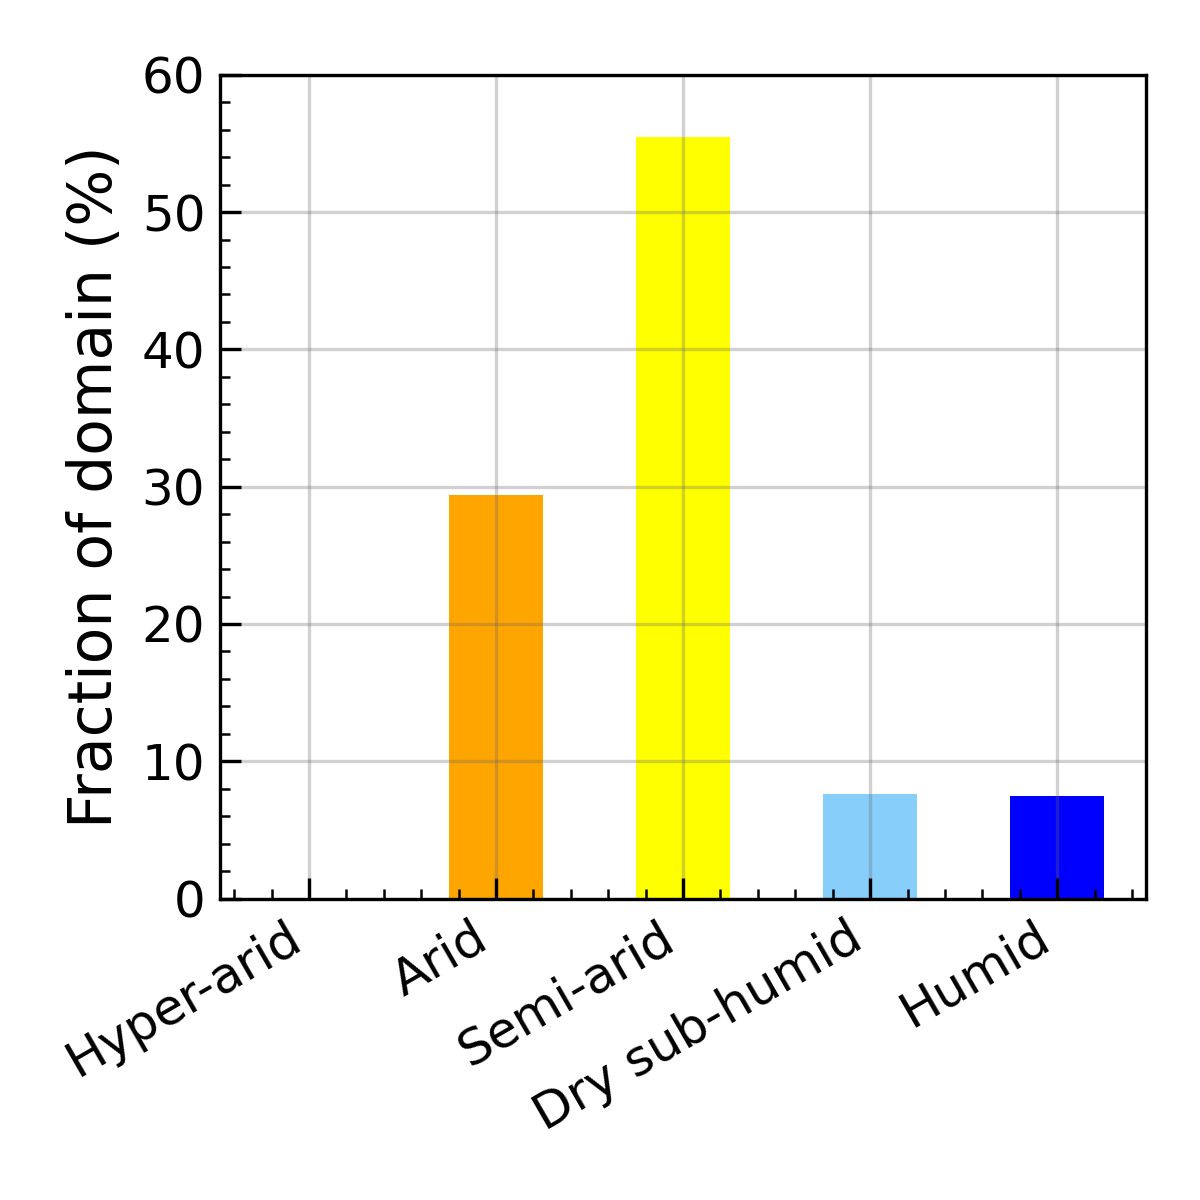
\includegraphics[width=\textwidth]{images/chap4/future/aridity_index_distribution_fut_irr.png}
    \end{subfigure}
    \caption{Spatial distribution of aridity index classes in the \presnoirr, \futnoirr, and \futirr simulations.}
    \label{fig:aridity_index_v2}
\end{figure}

%pres_no_irr
% Arid: 171 grid cells (18.566775244299674)
% semi-arid: 540 grid cells (58.63192182410424)
% Dry sub-humid: 58 grid cells (6.297502714440825)
% Humid: 152 grid cells (16.503800217155266)

%fut_no_irr
% Arid: 333 grid cells (36.156351791530945)
% semi-arid: 462 grid cells (50.1628664495114)
% Dry sub-humid: 63 grid cells (6.840390879478828)
% Humid: 63 grid cells (6.840390879478828)

%fut_irr
% Arid: 271 grid cells (29.42453854505972)
% semi-arid: 511 grid cells (55.48317046688383)
% Dry sub-humid: 70 grid cells (7.600434310532031)
% Humid: 69 grid cells (7.491856677524431)
